\newpage

\hypertarget{introduction}{%
\section{1. Introduction}\label{introduction}}

Depuis cette année, l'association INTech du campus rencontrait des
difficultés de gestion des impressions 3D faites par les membres. En
effet, depuis cette année, INTech offre aux membres du campus la
possibilité d'imprimer leur modèle 3D en devenant adhérents suivant le
processus décrit dans la figure 1.

Le processus commence lorsqu'un étudiant trouve un modèle 3D, le renomme
à son nom (au format \texttt{NOM-PRENOM.stl}) et remplit un Google Form
pour s'enregistrer dans un tableur, avant de lancer l'impression. Si
l'étudiant n'est pas présent à la fin du travail et que l'imprimante est
requise pour une autre tâche, un opérateur de l'association retire la
pièce et la stocke au local jusqu'au retour de l'étudiant qui vient
ensuite la récupérer. À la fin du mois, la phase de facturation
s'enclenche : l'opérateur consulte le tableur Google Sheets pour
calculer le montant total dû, crée un lien de paiement sur
\textbf{HelloAsso} et envoie la facture à l'étudiant. Si ce dernier paie
dans les 7 jours, l'opérateur valide la transaction dans sa
comptabilité, ce qui valide le succès du processus ; en revanche, s'il
ne règle pas sa dette après plusieurs relances de 7 jours et que le
plafond maximal d'avertissements est atteint, l'étudiant est inscrit sur
liste noire, ce qui entraîne l'échec de la procédure.

Actuellement, le système de gestion possède des problèmes. Les adhérents
doivent télécharger et paramétrer un logiciel appelé slicer qui permet
de transformer un modèle 3D en série d'instructions pour les imprimantes
3D, appelé G-code. On demande ensuite aux adhérents de charger le G-code
sur les imprimantes, de lancer les impressions et ensuite de remplir un
Google Form avec le nom de leur fichier, le poids de l'impression et
d'autres paramètres.

Ce système implique beaucoup d'étapes manuelles qui peuvent mener à des
erreurs et rendre la fraude facile. Il faut aussi former tout le monde
qui devient adhérent à l'utilisation des imprimantes.

\begin{figure}
\centering
\includesvg{diagrams/bpmn-before-diagram.svg}
\caption{Diagramme BPMN du fonctionnement pré-PrIntech}
\end{figure}

Intervient alors le projet PrINTech consistant au développement d'une
application web dynamique qui permette une gestion des impressions 3D de
manière automatique.

Contrairement à la solution existante, ce projet a une vision plus long
terme et facilite l'expansion à plus d'imprimantes ou de personnes et
permet de réduire la charge de travail du bureau.

\begin{center}\rule{0.5\linewidth}{0.5pt}\end{center}

\newpage

\hypertarget{terminologie}{%
\subsection{1.1. Terminologie}\label{terminologie}}

Pour faciliter la lecture de ce rapport, cette section regroupe et
définit les termes techniques, les acronymes et les notions spécifiques
au domaine de l'impression 3D et du développement web abordés dans ce
document.

\hypertarget{impression-3d-et-matuxe9riaux}{%
\subsubsection{Impression 3D et
Matériaux}\label{impression-3d-et-matuxe9riaux}}

\begin{itemize}
\tightlist
\item
  \textbf{Fichier STL (\texttt{.stl})} : Format de fichier standard en
  impression 3D (Stéréolithographie). Il représente la géométrie de la
  surface d'un objet 3D sous forme de triangles.
\item
  \textbf{Slicer (Trancheur)} : Logiciel qui découpe un modèle 3D
  virtuel en fines couches horizontales et génère les instructions
  nécessaires à l'imprimante.
\item
  \textbf{G-code} : Langage de programmation numérique universel utilisé
  pour piloter les machines-outils et les imprimantes 3D.
\item
  \textbf{Filament} : Le fil de plastique en bobine qui sert de
  ``matière première'' à l'imprimante 3D pour fabriquer les objets.
\item
  \textbf{PETG} : Un type de plastique très résistant (le même que celui
  des bouteilles d'eau, mais modifié), souvent utilisé pour des pièces
  qui doivent supporter des chocs ou rester en extérieur.
\item
  \textbf{PLA (Acide Polylactique)} : Plastique d'origine végétale
  couramment utilisé en impression 3D.
\item
  \textbf{Supports} : Structures temporaires imprimées en même temps que
  le modèle.
\end{itemize}

\hypertarget{technologies-web-architecture}{%
\subsubsection{Technologies Web \&
Architecture}\label{technologies-web-architecture}}

\begin{itemize}
\tightlist
\item
  \textbf{Angular} : Framework côté client (Frontend) utilisé pour
  concevoir une interface utilisateur dynamique.
\item
  \textbf{Django} : Framework de haut niveau basé sur Python, utilisé
  pour le développement de la logique métier (Backend).
\item
  \textbf{API REST} : Style d'architecture logicielle permettant au
  Frontend et au Backend de communiquer via le protocole HTTP.
\item
  \textbf{PostgreSQL} : Système de gestion de base de données
  relationnelle open-source.
\item
  \textbf{Docker \& Conteneurisation} : Technologie permettant d'isoler
  une application et ses dépendances dans un environnement virtuel
  appelé ``conteneur''.
\item
  \textbf{Nginx \& Gunicorn} : Duo de production où Nginx sert de
  serveur proxy inverse et Gunicorn de serveur d'application WSGI pour
  exécuter le code Python.
\end{itemize}

\hypertarget{outils-de-duxe9veloppement-tests}{%
\subsubsection{Outils de Développement \&
Tests}\label{outils-de-duxe9veloppement-tests}}

\begin{itemize}
\tightlist
\item
  \textbf{Git / Git Flow} : Git est le système de contrôle de version ;
  Git Flow est la méthodologie qui structure la collaboration (branches
  \texttt{main}, \texttt{develop}, \texttt{features/}).
\item
  \textbf{PR (Pull Request)} : Demande formelle de fusion de code
  soumise par un développeur pour relecture et validation.
\item
  \textbf{uv} : Gestionnaire de paquets et d'environnements Python
  extrêmement rapide écrit en Rust.
\item
  \textbf{Playwright} : Framework de test de bout en bout (E2E)
  permettant de simuler le comportement d'un utilisateur réel.
\end{itemize}

\newpage

\hypertarget{cahier-des-charges}{%
\section{2. Cahier des charges}\label{cahier-des-charges}}

À la suite des rapports et des échanges menés avec le bureau et les
membres actifs de l'association INTech, une analyse approfondie des
besoins opérationnels a été réalisée. Le constat est simple : le volume
croissant de demandes d'impression 3D sur le campus sature le modèle de
gestion actuel, basé sur des processus manuels et des outils tiers
(Google Forms, tableurs Sheets).

\hypertarget{description-du-sujet}{%
\subsection{2.1. Description du sujet}\label{description-du-sujet}}

Notre projet consiste en la réalisation d'une Application Web dynamique.
C'est-à-dire que le site doit être capable d'intéragir avec une base de
donnée qu'on doit aussi implémenter. Ce site web permettra alors
l'identification sécurisé des étudiants voulant imprimer des modèles 3D
avec un système de gestion d'utilisateurs, de requêtes, et de gestion de
queues. Cette plateforme aura pour objectifs principaux :

\begin{itemize}
\tightlist
\item
  \textbf{L'authentification sécurisée} des étudiants du campus
  souhaitant utiliser les services d'impression 3D.
\item
  \textbf{La gestion des utilisateurs} en distinguant les rôles
  (adhérents, bureau, membre d'un projet) et leurs droits associés.
\item
  \textbf{Le traitement des requêtes} afin de centraliser, suivre et
  historiser toutes les demandes de fabrication soumises par les élèves.
\item
  \textbf{La gestion des crédits et de la tarification} afin de
  permettre de payer chaque impression
\item
  \textbf{Espace administrateur} Interface d'administration pour une
  gestion complète
\end{itemize}

\newpage

\hypertarget{liste-des-fonctionnalituxe9s-de-lapplication}{%
\subsection{2.2. Liste des fonctionnalités de
l'application}\label{liste-des-fonctionnalituxe9s-de-lapplication}}

Afin de répondre au sujet, l'application doit intégrer les
fonctionnalités suivantes, classées par priorité de développement :

\begin{longtable}[]{@{}
  >{\raggedright\arraybackslash}p{(\columnwidth - 6\tabcolsep) * \real{0.0870}}
  >{\raggedright\arraybackslash}p{(\columnwidth - 6\tabcolsep) * \real{0.3261}}
  >{\raggedright\arraybackslash}p{(\columnwidth - 6\tabcolsep) * \real{0.4783}}
  >{\centering\arraybackslash}p{(\columnwidth - 6\tabcolsep) * \real{0.1087}}@{}}
\toprule\noalign{}
\begin{minipage}[b]{\linewidth}\raggedright
ID
\end{minipage} & \begin{minipage}[b]{\linewidth}\raggedright
Fonctionnalité de l'application
\end{minipage} & \begin{minipage}[b]{\linewidth}\raggedright
Description technique
\end{minipage} & \begin{minipage}[b]{\linewidth}\centering
Priorité
\end{minipage} \\
\midrule\noalign{}
\endhead
\bottomrule\noalign{}
\endlastfoot
\textbf{F01} & \textbf{Authentification} & Connexion et déconnexion. &
Haute \\
\textbf{F02} & \textbf{Gestion des profils} & Affichage et modification
des informations utilisateurs. & Basse \\
\textbf{F03} & \textbf{Gestion des impressions} & Flux complet
d'impression 3D, du dépôt STL à la mise en file. & Haute \\
\textbf{F03-1} & \textbf{Déposer un STL} & Upload d'un fichier STL. &
Haute \\
\textbf{F03-2} & \textbf{Slicer automatique} & Convertir le modèle en
G-code via un slicer. & Moyenne \\
\textbf{F03-3} & \textbf{Estimation du coût} & Calculer le prix
d'impression à partir des paramètres. & Basse \\
\textbf{F03-4} & \textbf{Position dans la file} & Afficher la place du
travail dans la file. & Basse \\
\textbf{F03-5} & \textbf{Priorité projets INTech} & Chaque utilisateur à
un rôle (adhérents, bureau, membre d'un projet) pour priiser les
impressions. & Basse \\
\textbf{F03-6} & \textbf{Crédit restant} & Afficher le crédit restant
d'un utilisateur. & Basse \\
\textbf{F03-7} & \textbf{Quantité d'impressions} & Indiquer le nombre
d'exemplaires à imprimer. & Basse \\
\textbf{F04} & \textbf{Espace administrateur} & Interface
d'administration pour une gestion complète. & Moyenne \\
\textbf{F04-1} & \textbf{Gestion des utilisateurs} & Créer, modifier et
supprimer les utilisateurs. & Haute \\
\textbf{F04-2} & \textbf{Gestion des travaux} & Créer, modifier et
supprimer la file de travaux. & Moyenne \\
\textbf{F04-3} & \textbf{Reprise des erreurs} & Déclarer un travail en
erreur et le remettre en file. & Moyenne \\
\textbf{F04-4} & \textbf{Gestion crédit} & Gestion des crédits des
utilisateurs dont la recharge de crédits. & Haute \\
\textbf{F05} & \textbf{Intégrations} & SSO et notifications externes. &
Pour aller plus loin \\
\textbf{F05-1} & \textbf{Intégration CAS} & Inscription et connexion via
le CAS de l'école. & Pour aller plus loin \\
\textbf{F05-2} & \textbf{Intégration Discord} & Utiliser des webhooks
pour les notifications. & Pour aller plus loin \\
\textbf{F05-3} & \textbf{Intégration HelloAsso} & Créditer les comptes
via HelloAsso. & Pour aller plus loin \\
\textbf{F06} & \textbf{Impression technique} & Options avancées
d'impression. & Pour aller plus loin \\
\textbf{F06-1} & \textbf{Utilisation de supports} & Détecter quand
l'utilisation de supports est nécessaire. & Pour aller plus loin \\
\textbf{F06-2} & \textbf{Paramétrage du slicer} & Permettre l'upload
d'un JSON de paramètres. & Pour aller plus loin \\
\textbf{F06-3} & \textbf{Choix des matériaux} & Choisir un plastique
autre que le PLA. & Pour aller plus loin \\
\textbf{F07} & \textbf{Gestion des filaments} & Administration des
filaments et du stock. & Pour aller plus loin \\
\textbf{F07-1} & \textbf{Activation des filaments} & Activer et
désactiver des filaments. & Pour aller plus loin \\
\textbf{F07-2} & \textbf{Gestion des filament} & Gérer la quantité de
filament restant. & Pour aller plus loin \\
\textbf{F07-3} & \textbf{Gestion de consommation} & Rapport sur
quantités, crédits et montant imprimé. & Pour aller plus loin \\
\end{longtable}

\begin{center}\rule{0.5\linewidth}{0.5pt}\end{center}

\newpage

\hypertarget{conception}{%
\section{3. Conception}\label{conception}}

\hypertarget{base-de-donnuxe9es}{%
\subsection{3.1. Base de données}\label{base-de-donnuxe9es}}

Comme l'illustre ce schema, lorsqu'un User (caractérisé par un rôle
applicatif et un solde de crédits) souhaite fabriquer un objet, il émet
une demande d'impression (Request). Celle-ci encapsule un fichier
numérique (File) contenant le modèle 3D et ses paramètres de découpage
en format JSON (para\_slicer), lui-même associé à un consommable précis
(Filament) défini par son type (PLA ou PETG) et sa couleur. La demande
est ensuite affectée à une machine (Printer) identifiée par son modèle
et son état de disponibilité. Enfin, pour éradiquer les risques de
fraude et automatiser la comptabilité, chaque transaction (recharge de
compte par carte/espèces ou débit/remboursement lié à une impression)
est tracée par l'entité Operation. Cette table lie un agent du bureau à
un utilisateur bénéficiaire tout en restant historiquement connectée à
la Request d'origine.

\begin{figure}
\centering
\includesvg{diagrams/db-diagram.svg}
\caption{Schema de base de données}
\end{figure}

\begin{center}\rule{0.5\linewidth}{0.5pt}\end{center}

\newpage

\hypertarget{suxe9quence-de-lauthentification}{%
\subsection{3.2. Séquence de
l'Authentification}\label{suxe9quence-de-lauthentification}}

Pour sécuriser l'accès aux ressources de la plateforme et garantir que
chaque étudiant interagit uniquement avec ses propres données, le projet
implémente un flux d'authentification basé sur des jetons d'accès (JWT)
via la librairie Django REST Framework SimpleJWT. Ce mécanisme élimine
les failles de sécurité de l'ancien système et permet une communication
fluide entre le Frontend Angular et l'API Backend.

Le diagramme de séquence suivant détaille les phases d'inscription, de
connexion et de renouvellement des jetons :

\begin{figure}
\centering
\includesvg{diagrams/auth-diagram.svg}
\caption{Schema de l'authentification}
\end{figure}

\begin{center}\rule{0.5\linewidth}{0.5pt}\end{center}

\newpage

\hypertarget{processus-dimpression-3d-avec-printech}{%
\subsection{3.3. Processus d'impression 3D avec
PrIntech}\label{processus-dimpression-3d-avec-printech}}

\hypertarget{description-du-processus-dimpression-3d}{%
\subsubsection{Description du processus d'impression
3D}\label{description-du-processus-dimpression-3d}}

Le processus débute lorsqu'un étudiant dépose un modèle 3D sur la
plateforme (\textbf{F03-1 : Déposer un STL}). Une fois la requête
enregistrée dans l'interface d'administration (\textbf{F04-2 : Gestion
des travaux}), le système évalue automatiquement les ressources
nécessaires. Il vérifie d'une part la quantité de matière disponible
(\textbf{F07-2 : Gestion des filaments}) et d'autre part le montant
estimé de l'impression (\textbf{F03-3 : Estimation du coût}) par rapport
aux ressources financières de l'utilisateur (\textbf{F03-6 : Crédit
restant}). Si le plastique est manquant ou indisponible, la demande est
arrêtée. Si l'utilisateur ne dispose pas de fonds suffisants,
l'application le redirige vers le module externe afin de renflouer son
compte (\textbf{F05-3 : Intégration HelloAsso}).

Dès que ces vérifications sont validées, le travail rejoint la file
d'attente informatique et l'opérateur lui attribue une machine
disponible (\textbf{F04-2 : Gestion des travaux}), tout en prenant en
compte le rôle de l'utilisateur (\textbf{F03-5 : Priorité projets
INTech}). L'application procède alors au prélèvement des fonds requis
sur le compte de l'étudiant (\textbf{F04-4 : Gestion crédit}), met à
jour le statut informatique de l'imprimante, et l'opérateur lance
physiquement la fabrication de la pièce (\textbf{F03 : Gestion des
impressions}). À la fin du cycle, deux situations peuvent se présenter :
* \textbf{En cas de succès :} l'opérateur valide la fin de la tâche
(\textbf{F04-2 : Gestion des travaux}), l'imprimante repasse
informatiquement à l'état disponible, le stock de plastique restant est
ajusté (\textbf{F07-2 : Gestion des filaments}) et une alerte
automatisée est envoyée à l'étudiant (\textbf{F05-2 : Intégration
Discord}) pour qu'il vienne récupérer sa pièce. * \textbf{En cas d'échec
:} l'opérateur déclare l'avarie sur l'interface (\textbf{F04-3 : Reprise
des erreurs}), libérant immédiatement la machine. Le système réajuste
alors automatiquement le solde de l'étudiant (\textbf{F04-4 : Gestion
crédit}) tout en envoyant une notification pour l'avertir du problème
(\textbf{F05-2 : Intégration Discord}).

\begin{figure}
\centering
\includesvg{diagrams/bpmn-after-diagram.svg}
\caption{Diagramme BPMN du fonctionnement post-PrIntech}
\end{figure}

\begin{center}\rule{0.5\linewidth}{0.5pt}\end{center}

\newpage

\hypertarget{ruxe9alisation-et-choix-techniques}{%
\section{4. Réalisation et choix
techniques}\label{ruxe9alisation-et-choix-techniques}}

\hypertarget{choix-des-technologies}{%
\subsection{4.1. Choix des technologies}\label{choix-des-technologies}}

Les technologies pour développer une Application Web sont nombreuses.
Pour faire la sélection des technologies, nous avons d'abord examiné
lesquelles étaient capables de répondre à notre cahier des charges, puis
ensuite sur les technologies auxquelles les membres de notre équipe
avaient déjà de l'expérience. Sur la base de ces critères, nous avons
sélectionné le stack suivant. D'abord pour le frontend :

\begin{itemize}
\tightlist
\item
  \textbf{Angular} : Pour la réalisation de l'interface utilisateur.
  Angular s'appuie sur l'architecture de composants et sur le langage
  \textbf{TypeScript}. Ce choix apporte un typage fort, une structure
  rigoureuse.
\end{itemize}

Ensuite pour le backend :

\begin{itemize}
\item
  \textbf{Django (Python)} : Utilisé pour développer le cœur logique du
  backend et l'API REST (via \emph{Django REST Framework}).
\item
  \textbf{uv} : Afin de gérer nos librairies et versions de python, on a
  utilisé uv. C'est un équivalent de poetry mais en plus optimisé car
  implémenté en Rust. On doit alors préciser avant chaque commande ``uv
  run'' afin que le processus passe bien par uv.
\item
  \textbf{Swagger (OpenAPI)} : Intégré à notre backend pour la
  documentation et le test de l'API REST. Swagger génère automatiquement
  une interface web interactive à partir des routes de notre application
  Django. Cela permet aux développeurs frontend de comprendre
  instantanément les points de terminaison (\emph{endpoints}), les
  paramètres attendus et les réponses de l'API, facilitant ainsi
  grandement la communication et l'intégration entre le frontend et le
  backend.
\item
  \textbf{PostgreSQL} : Ce système de gestion de base de données
  relationnelle (SGBDR) open-source a été retenu pour sa robustesse, sa
  conformité ACID et sa gestion fine des transactions financières
  (crédits, remboursements, opérations). Sa capacité à indexer
  efficacement les données structurées garantit des performances
  optimales lors de la montée en charge du système et du suivi des files
  d'attente de travaux.
\item
  \textbf{Klipper} : comme firmware des imprimantes. Ce firmware
  communautaire vient remplacer celui du constructeur
\item
  \textbf{Moonraker} : expose les API JSON-RPC de Klipper avec une API
  REST
\item
  \textbf{FDM Monster} Cet orchestrateur open-source centralise la
  gestion d'une flotte d'imprimantes 3D. Connecté aux différentes
  instances Moonraker, il permet de piloter le parc, de centraliser le
  contrôle des machines et de gérer globalement les files d'attente
  d'impression.
\end{itemize}

\hypertarget{tests-validation-et-qualituxe9-logicielle}{%
\subsubsection{Tests, Validation et Qualité
Logicielle}\label{tests-validation-et-qualituxe9-logicielle}}

\begin{itemize}
\tightlist
\item
  \textbf{Tests natifs Django (TestCase)} : Intégrés directement au
  backend, le framework de test unitaire et d'intégration natif de
  Django permet de sécuriser l'intégrité de la base de données lors des
  transactions critiques. Ils valident de manière isolée les calculs de
  prix, l'exactitude des débits et remboursements de crédits, le respect
  des rôles utilisateurs pour la gestion des priorités, ainsi que les
  transitions de statut des requêtes d'impression (du dépôt initial
  jusqu'à la mise en file).
\item
  \textbf{Playwright} : Framework moderne retenu pour l'automatisation
  des tests de bout en bout (\emph{End-to-End}). Complémentaire aux
  tests Django, Playwright nous permet de simuler le parcours complet
  d'un utilisateur sur un navigateur réel de manière isolée.
\end{itemize}

\hypertarget{conteneurisation-et-infrastructure}{%
\subsubsection{Conteneurisation et
Infrastructure}\label{conteneurisation-et-infrastructure}}

\begin{itemize}
\tightlist
\item
  \textbf{Docker \& Docker Compose} : Afin de partitionner logiquement
  les différentes couches applicatives (Frontend, Backend, Base de
  données), nous avons conteneurisé chaque service. Technologie
  incontournable dans le milieu professionnel, Docker garantit que
  l'application s'exécute de manière strictement identique sur les
  machines de développement des développeurs et sur le serveur de
  production, simplifiant ainsi drastiquement la configuration de
  l'infrastructure.
\item
  \textbf{Nginx \& Gunicorn} : Pour le déploiement en production,
  \textbf{Gunicorn} fait office de serveur d'application WSGI, chargé
  d'exécuter le code Python/Django en gérant efficacement les requêtes
  concurrentes via un système de processus de travail (\emph{workers}).
  Il est placé derrière \textbf{Nginx}, configuré comme un proxy inverse
  (\emph{reverse proxy}). Nginx assure la sécurité globale, gère les
  certificats SSL/TLS (HTTPS), sert directement les fichiers statiques
  et médias lourds (comme les fichiers STL stockés), et distribue la
  charge vers l'application backend.
\end{itemize}

\hypertarget{outils-de-duxe9veloppement-et-de-collaboration}{%
\subsubsection{Outils de développement et de
collaboration}\label{outils-de-duxe9veloppement-et-de-collaboration}}

\begin{itemize}
\tightlist
\item
  \textbf{Visual Studio Code (VS Code)} : Choisi comme environnement de
  développement intégré (IDE) principal par l'équipe. Il offre une
  intégration native de Git, et des extensions pour Python/Django et
  Angular.
\item
  \textbf{Git \& GitFlow} : Pour la gestion de version, nous utilisons
  \textbf{Git} hébergé sur \textbf{GitHub}. Afin d'organiser le travail
  collaboratif de l'équipe sans bloquer la production, nous appliquons
  la méthodologie \textbf{GitFlow}. Cette approche structure notre dépôt
  en plusieurs branches strictes : \texttt{main} pour les versions
  stables, \texttt{develop} pour centraliser les fonctionnalités prêtes,
  et des branches \texttt{feature/} isolées pour chaque développeur.
\item
  \textbf{Discord \& Webhooks GitHub} : Discord est notre outil central
  de communication d'équipe. Pour automatiser notre suivi de projet,
  nous y avons configuré des \textbf{webhooks GitHub}. À chaque fois
  qu'un développeur pousse du code (\emph{push}), ouvre une demande de
  fusion (\emph{pull request}) , une notification automatique est
  envoyée dans un salon dédié sur Discord. Cela permet un suivi de
  l'avancement facile.
\end{itemize}

\begin{center}\rule{0.5\linewidth}{0.5pt}\end{center}

\newpage

\hypertarget{ruxe9alisation}{%
\subsection{4.2. Réalisation}\label{ruxe9alisation}}

Pour la conteneurisation, il a fallu créer les conteneurs. Pour se
faire, il faut configurer un fichier ``docker-compose.yaml'' afin qu'il
créer un conteneur PostgreSQL configuré sur le bon port après la
commande.

Enfin pour la mise en commun du code, on a utilisé Git, et plus
particulièrement git flow qui permet de produire simplement un cadre de
travail professionnel (avec les branches main, develop,
features/\ldots{} etc.) et des commandes qui facilitent son utilisation.

Afin de valider l'expérience utilisateur et de documenter le rendu final
de notre application PrIntech, cette section présente les principales
interfaces développées. Les captures d'écran sont structurées selon les
deux grands espaces de la plateforme : l'espace adhérent (client) et
l'espace d'administration (opérateur).

\hypertarget{espace-utilisateur-et-authentification}{%
\subsubsection{4.2.1. Espace Utilisateur et
Authentification}\label{espace-utilisateur-et-authentification}}

Cet espace regroupe les écrans accessibles par les étudiants du campus
pour gérer leur compte et soumettre leurs impressions.

\begin{itemize}
\item
  \textbf{Interface de Connexion}
  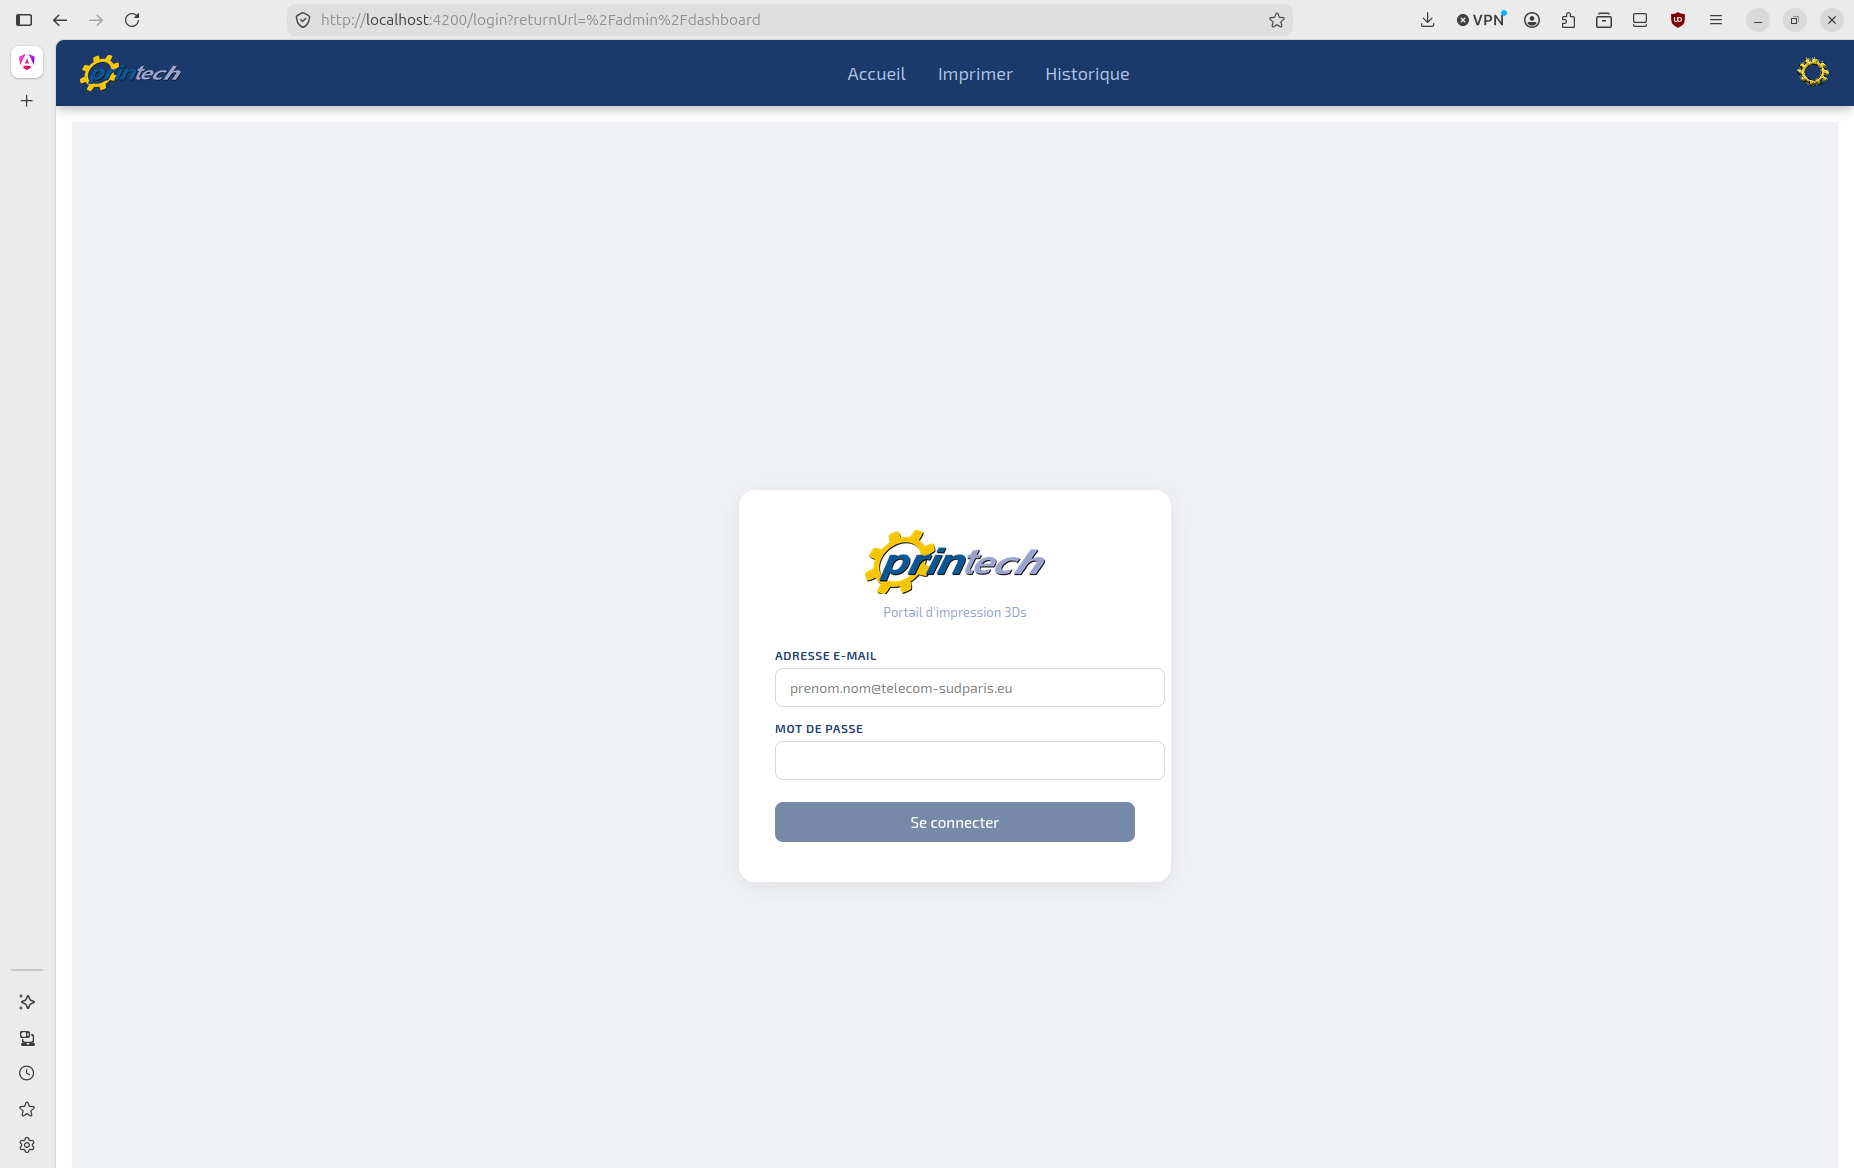
\includegraphics{screenshots/login.png}\\
  Cette interface épurée permet l'authentification sécurisée des
  utilisateurs (Fonctionnalité \textbf{F01}).
\item
  \textbf{Page d'Accueil} 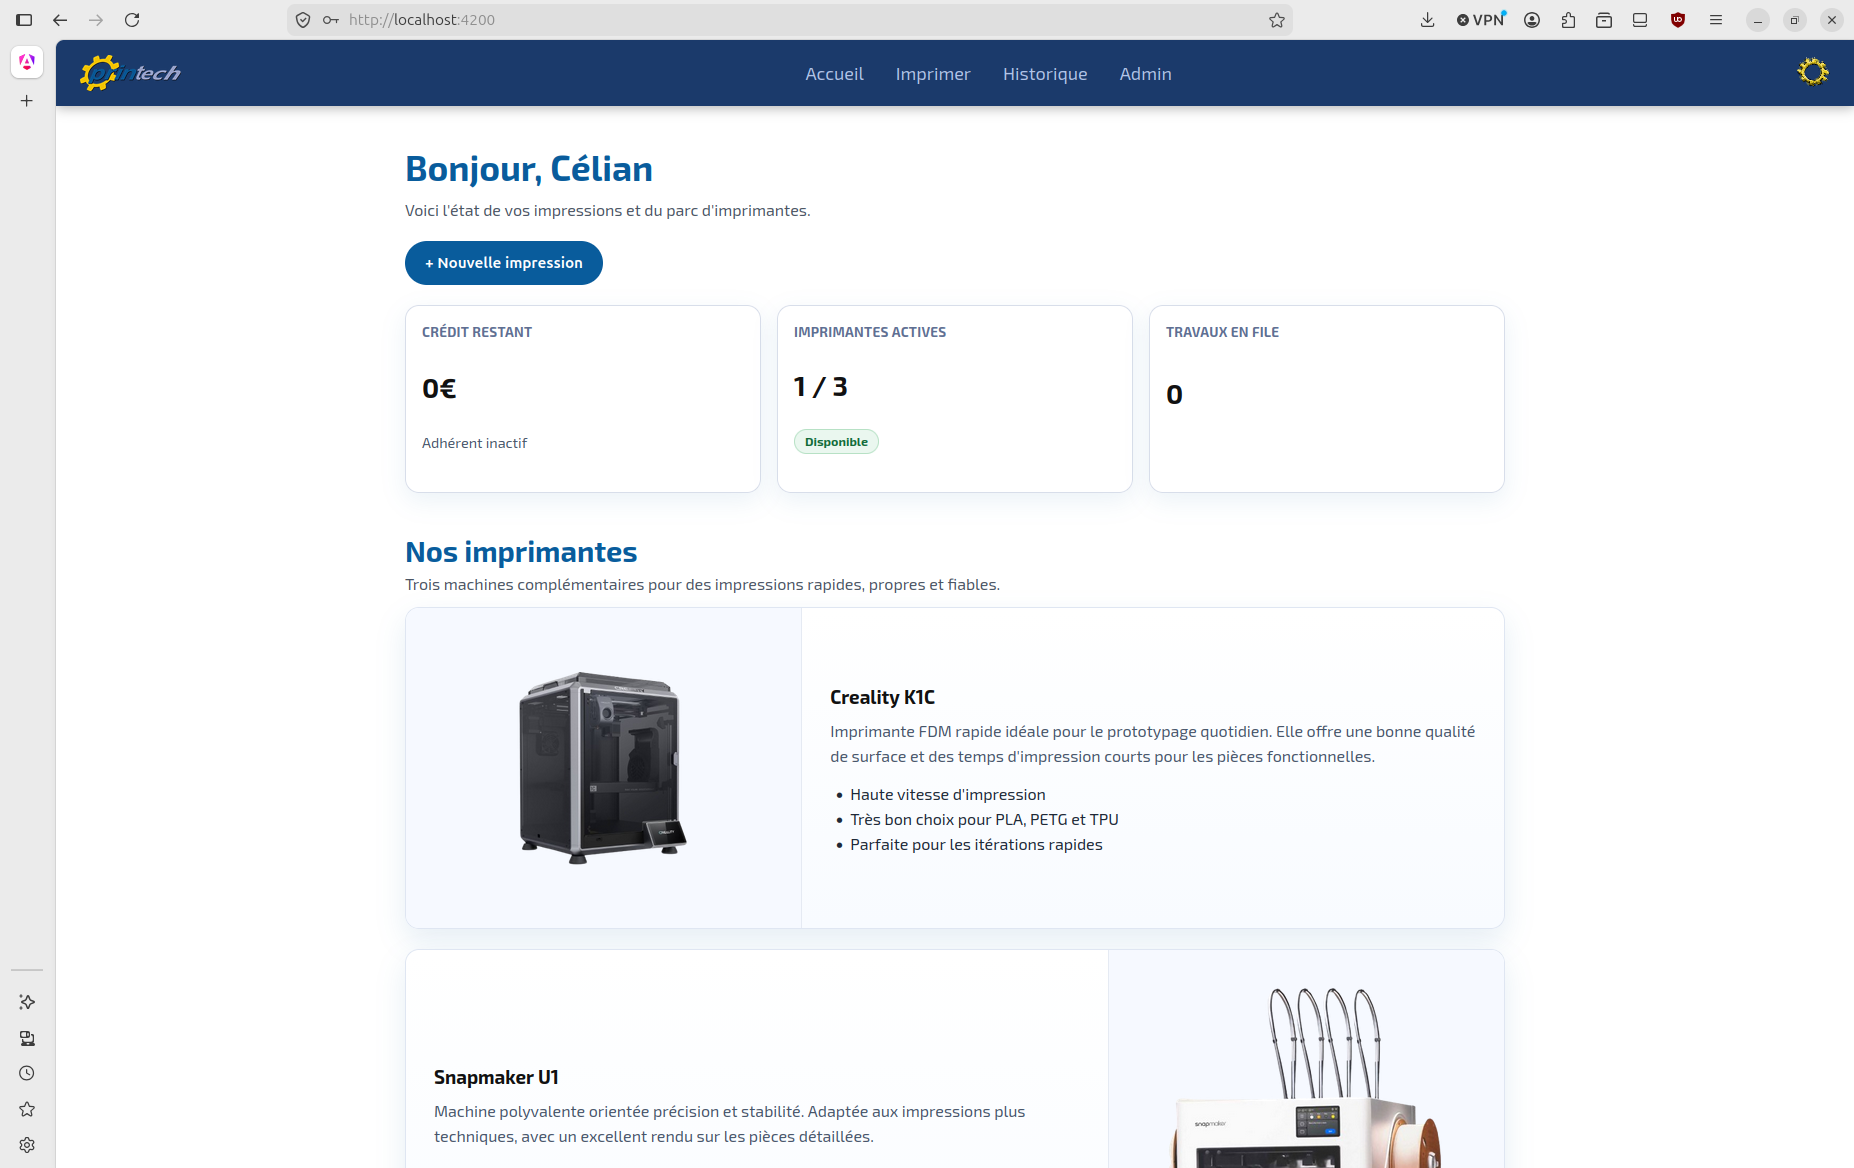
\includegraphics{screenshots/home.png}\\
  Le tableau de bord principal de l'étudiant. Il offre une vue
  d'ensemble claire sur ses activités courantes, son solde mis en valeur
  (Fonctionnalité \textbf{F03-6 : Crédit restant}).
\item
  \textbf{Dépôt d'une demande d'impression}
  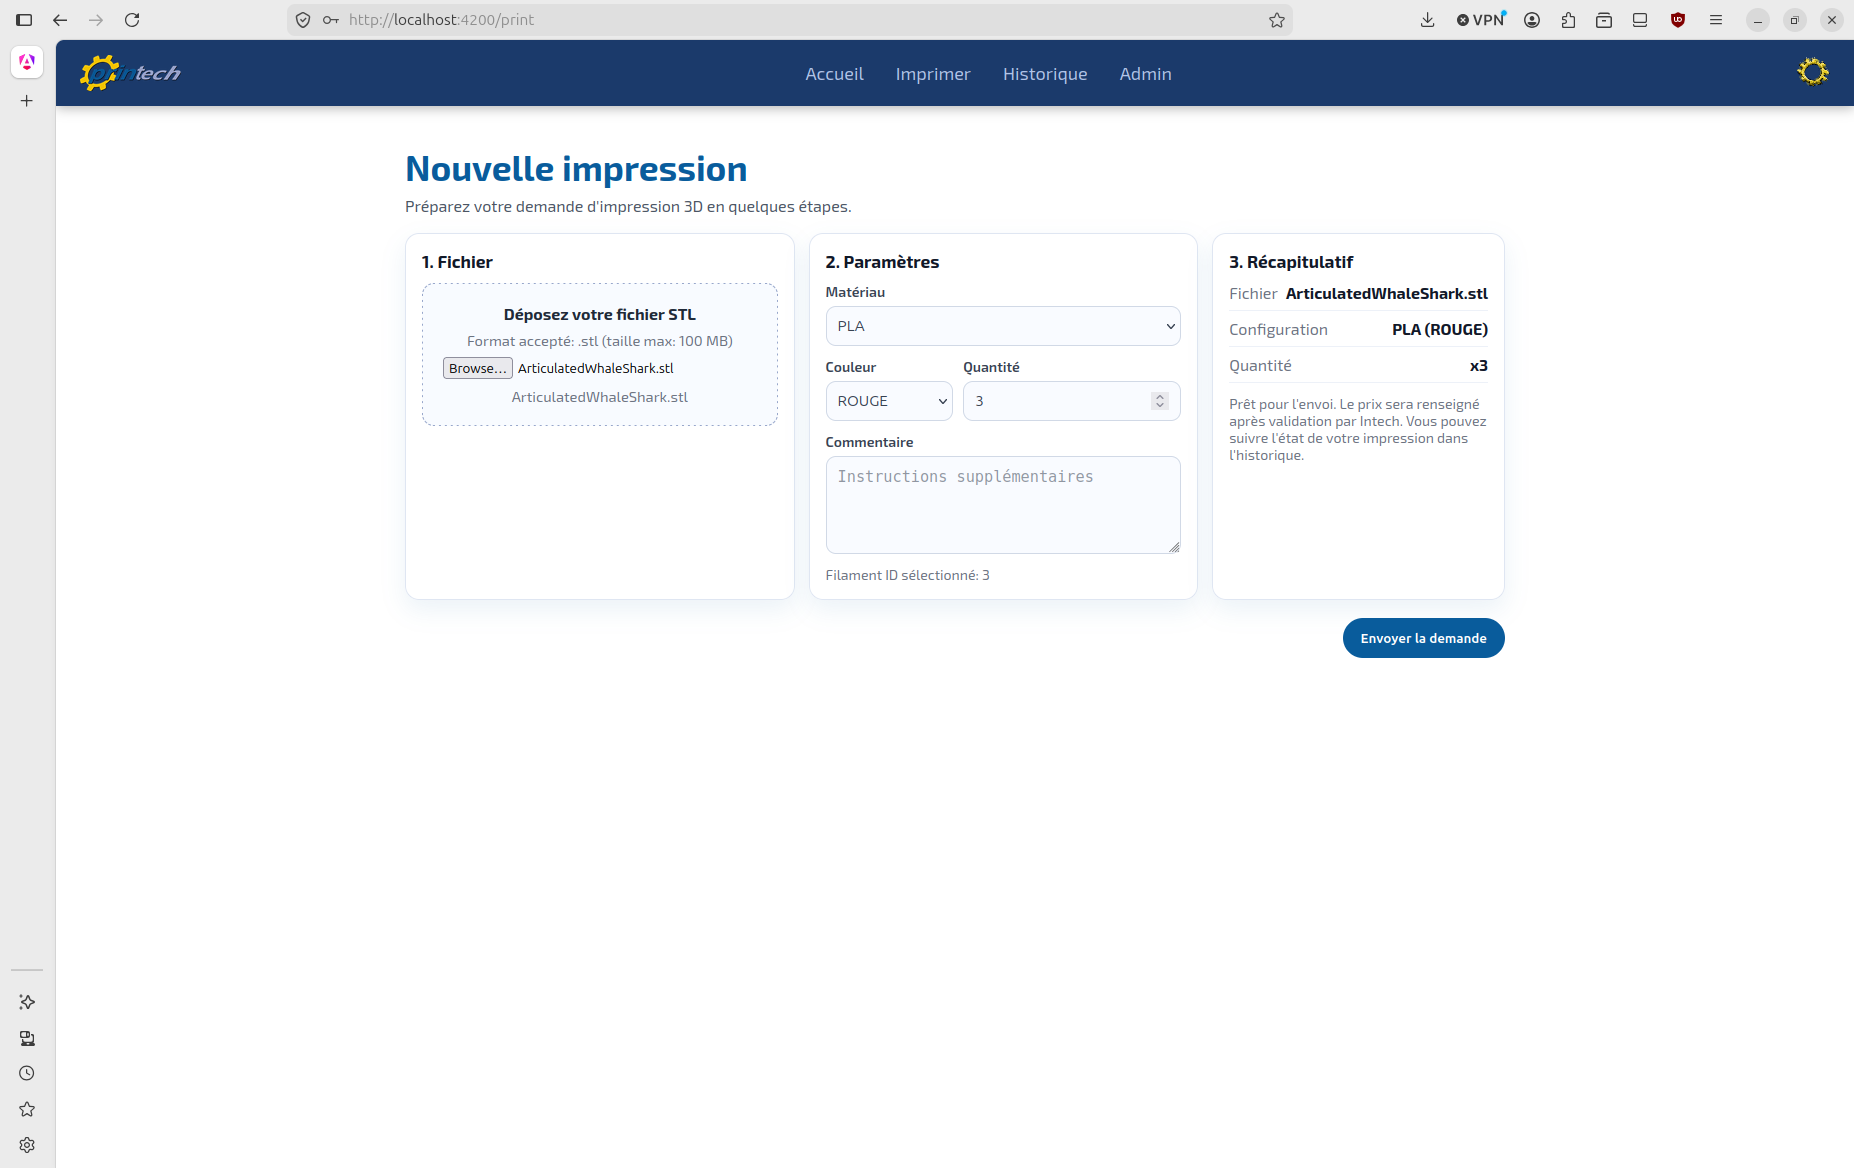
\includegraphics{screenshots/request.png}\\
  Formulaire intuitif dédié au dépôt des fichiers 3D (Fonctionnalité
  \textbf{F03-1 : Déposer un STL}). L'étudiant peut y téléverser son
  modèle, spécifier la quantité d'exemplaires souhaitée (\textbf{F03-7})
  ainsi que le choix des matériaux avant l'envoi au serveur.
\item
  \textbf{Historique des travaux}
  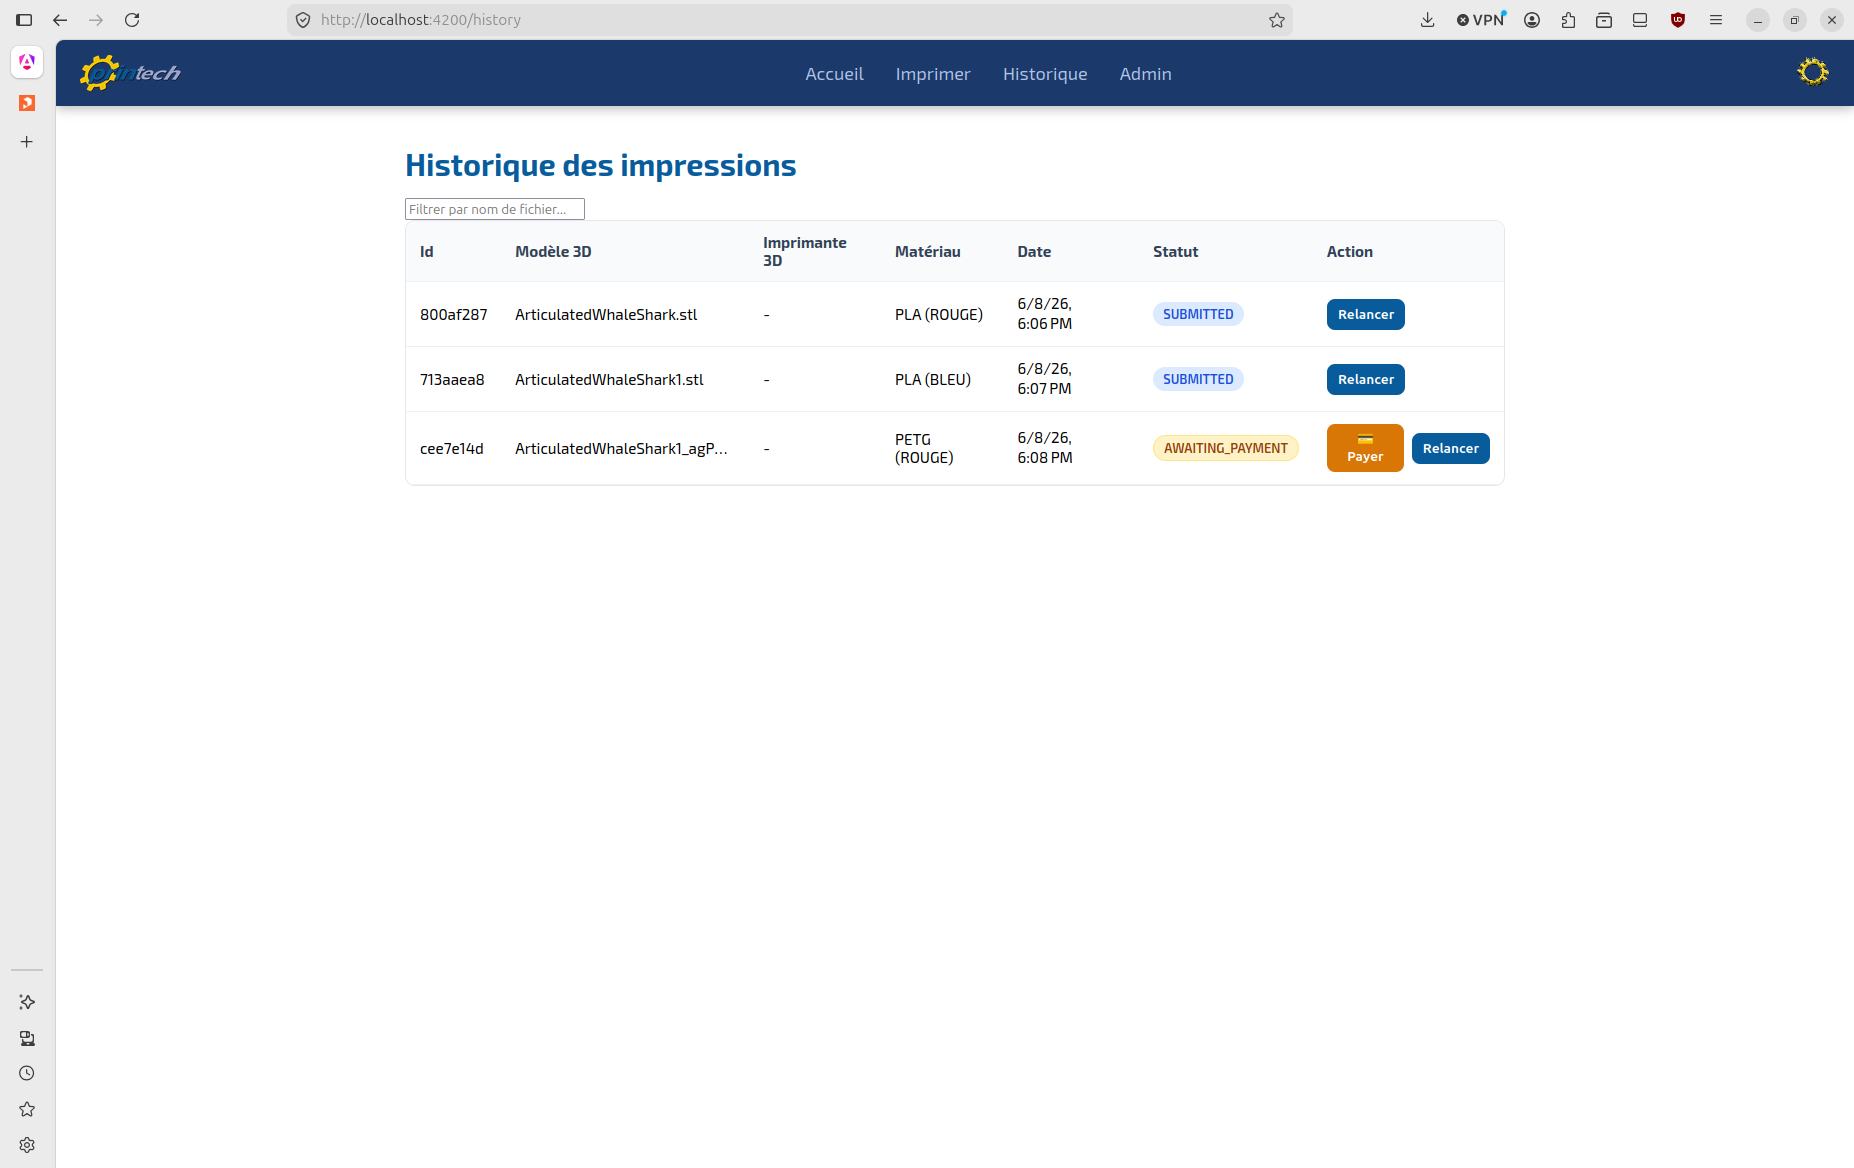
\includegraphics{screenshots/historique.png}\\
  Cette vue liste l'intégralité des commandes passées par l'étudiant.
  (\textbf{F03-4 : Position dans la file}).
\end{itemize}

\begin{center}\rule{0.5\linewidth}{0.5pt}\end{center}

\hypertarget{espace-administration-et-gestion-des-opuxe9rations}{%
\subsubsection{4.2.2. Espace Administration et Gestion des
Opérations}\label{espace-administration-et-gestion-des-opuxe9rations}}

Réservé aux membres du bureau et aux opérateurs de l'association INTech
(Fonctionnalité \textbf{F04}), cet espace permet un pilotage complet du
service et du parc matériel.

\begin{itemize}
\item
  \textbf{Gestion de la file des travaux}
  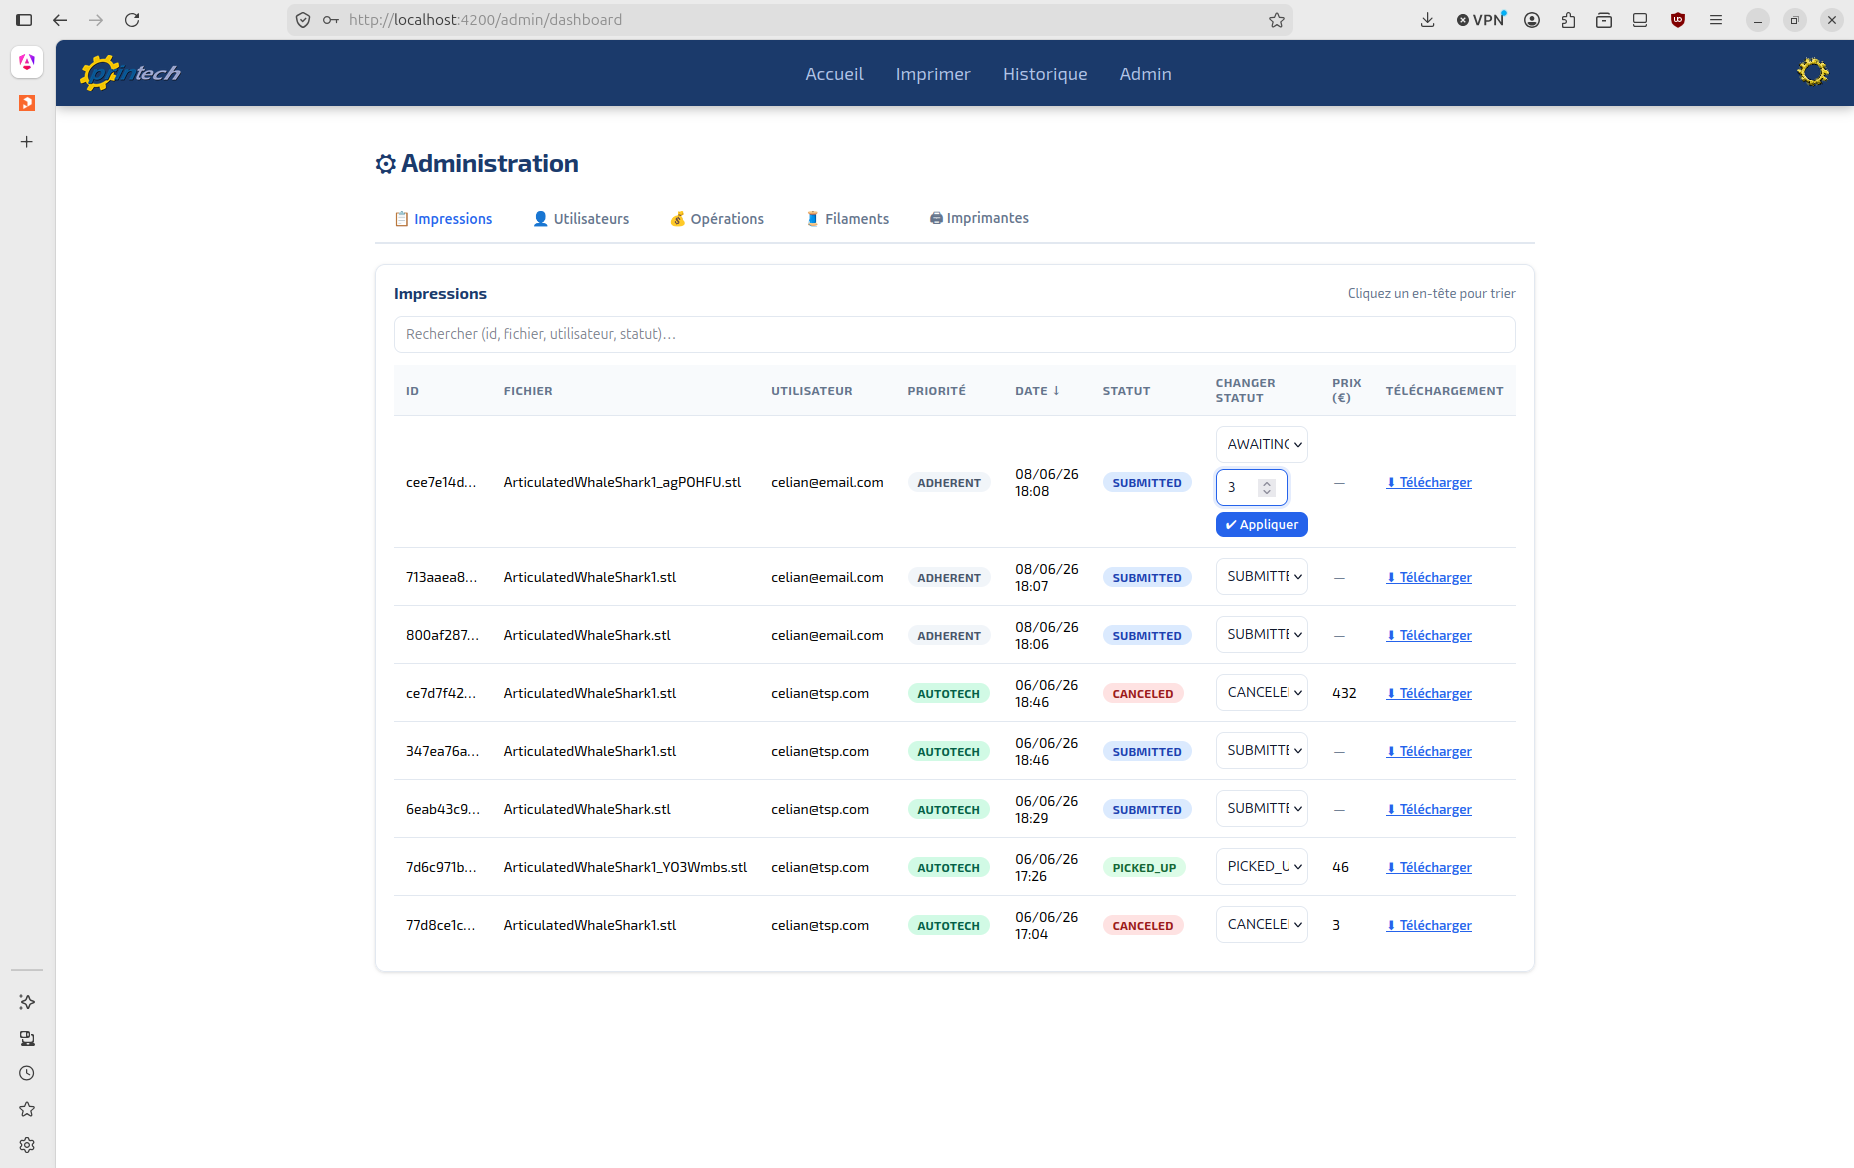
\includegraphics{screenshots/admin-requests.png}\\
  Interface maîtresse de l'opérateur (Fonctionnalité \textbf{F04-2 :
  Gestion des travaux}). Elle centralise les fichiers \texttt{.stl}
  soumis, permet d'assigner manuellement ou automatiquement une
  imprimante libre et d'appliquer la tarification calculée.
\item
  \textbf{Suivi du parc d'imprimantes}
  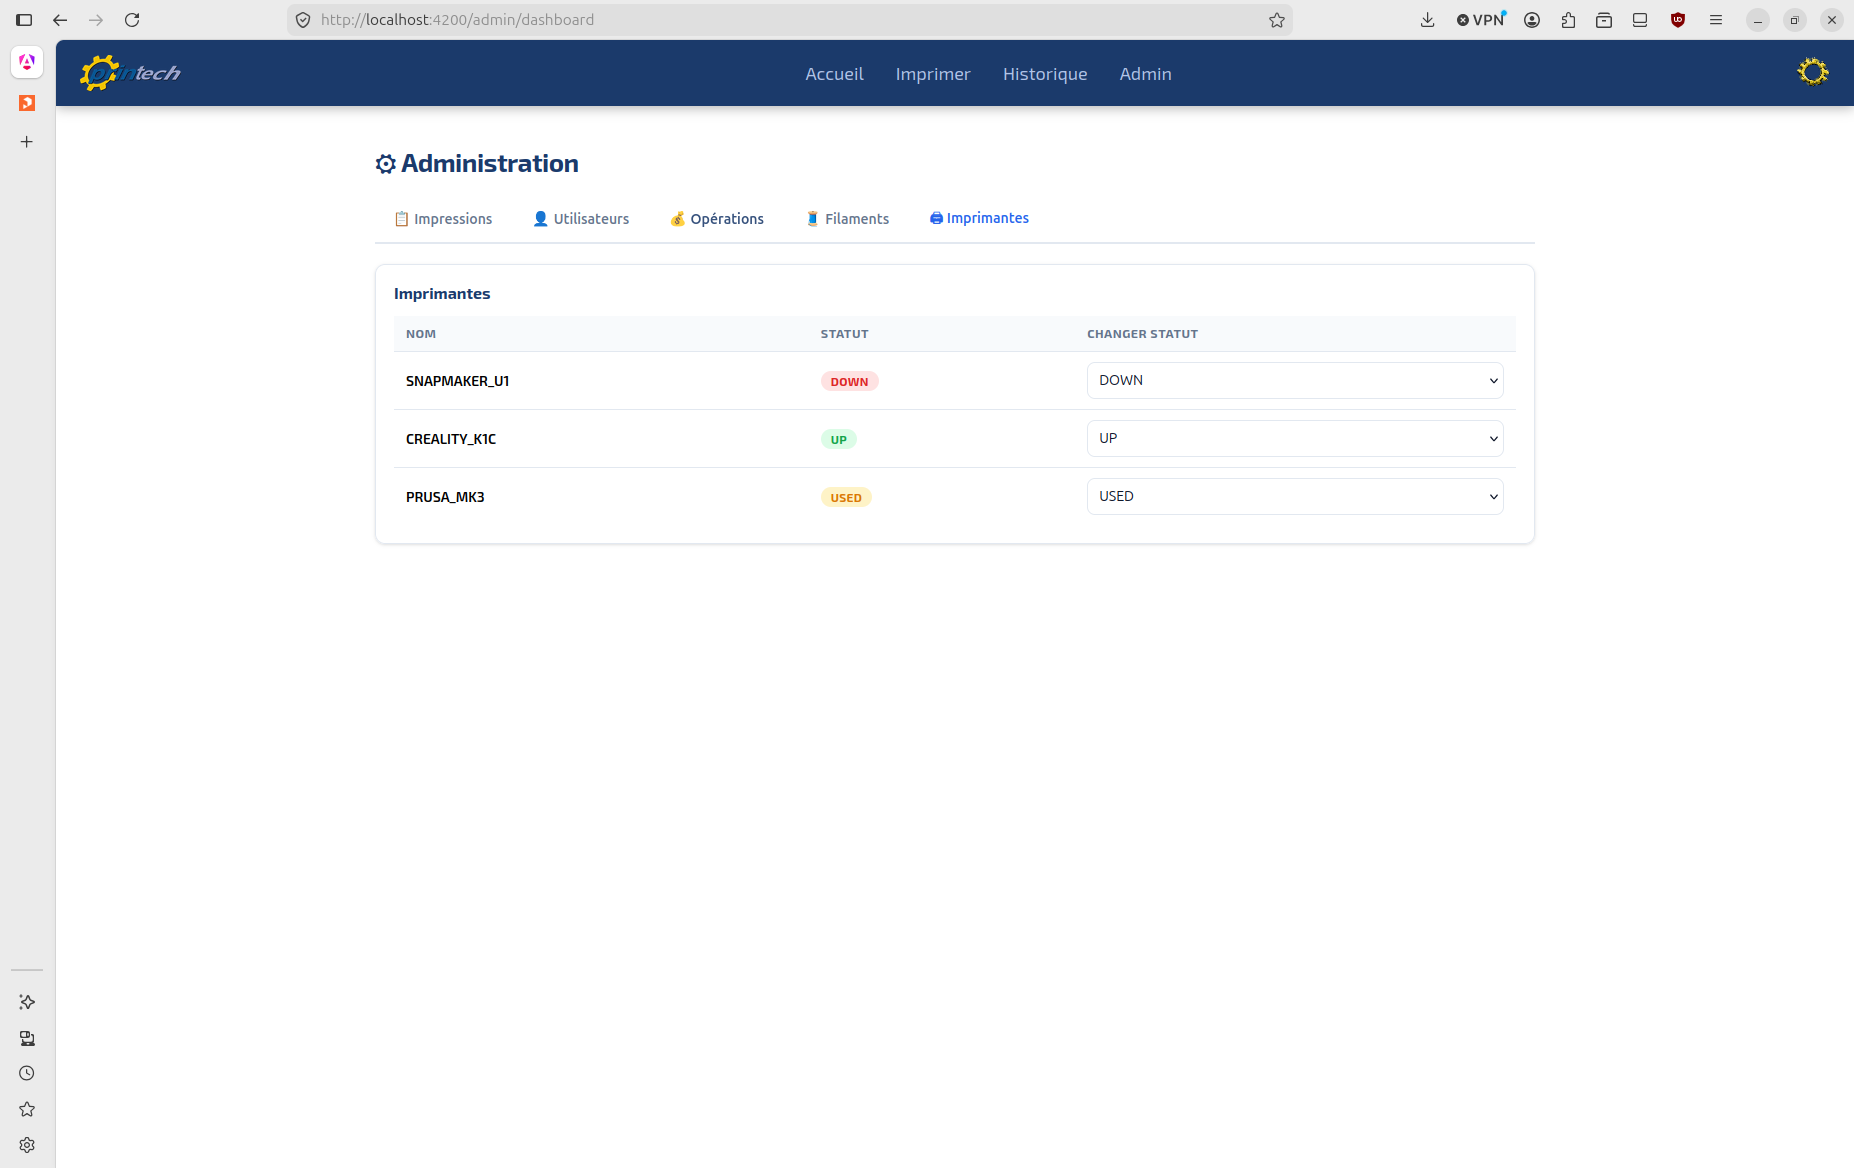
\includegraphics{screenshots/admin-printers.png}\\
  Écran de supervision du statut des machines connectées.
  L'administrateur peut visualiser instantanément quelles machines sont
  disponibles (\texttt{UP}), occupées (\texttt{USED}) ou hors service
  (\texttt{DOWN}).
\item
  \textbf{Gestion des stocks de consommables}
  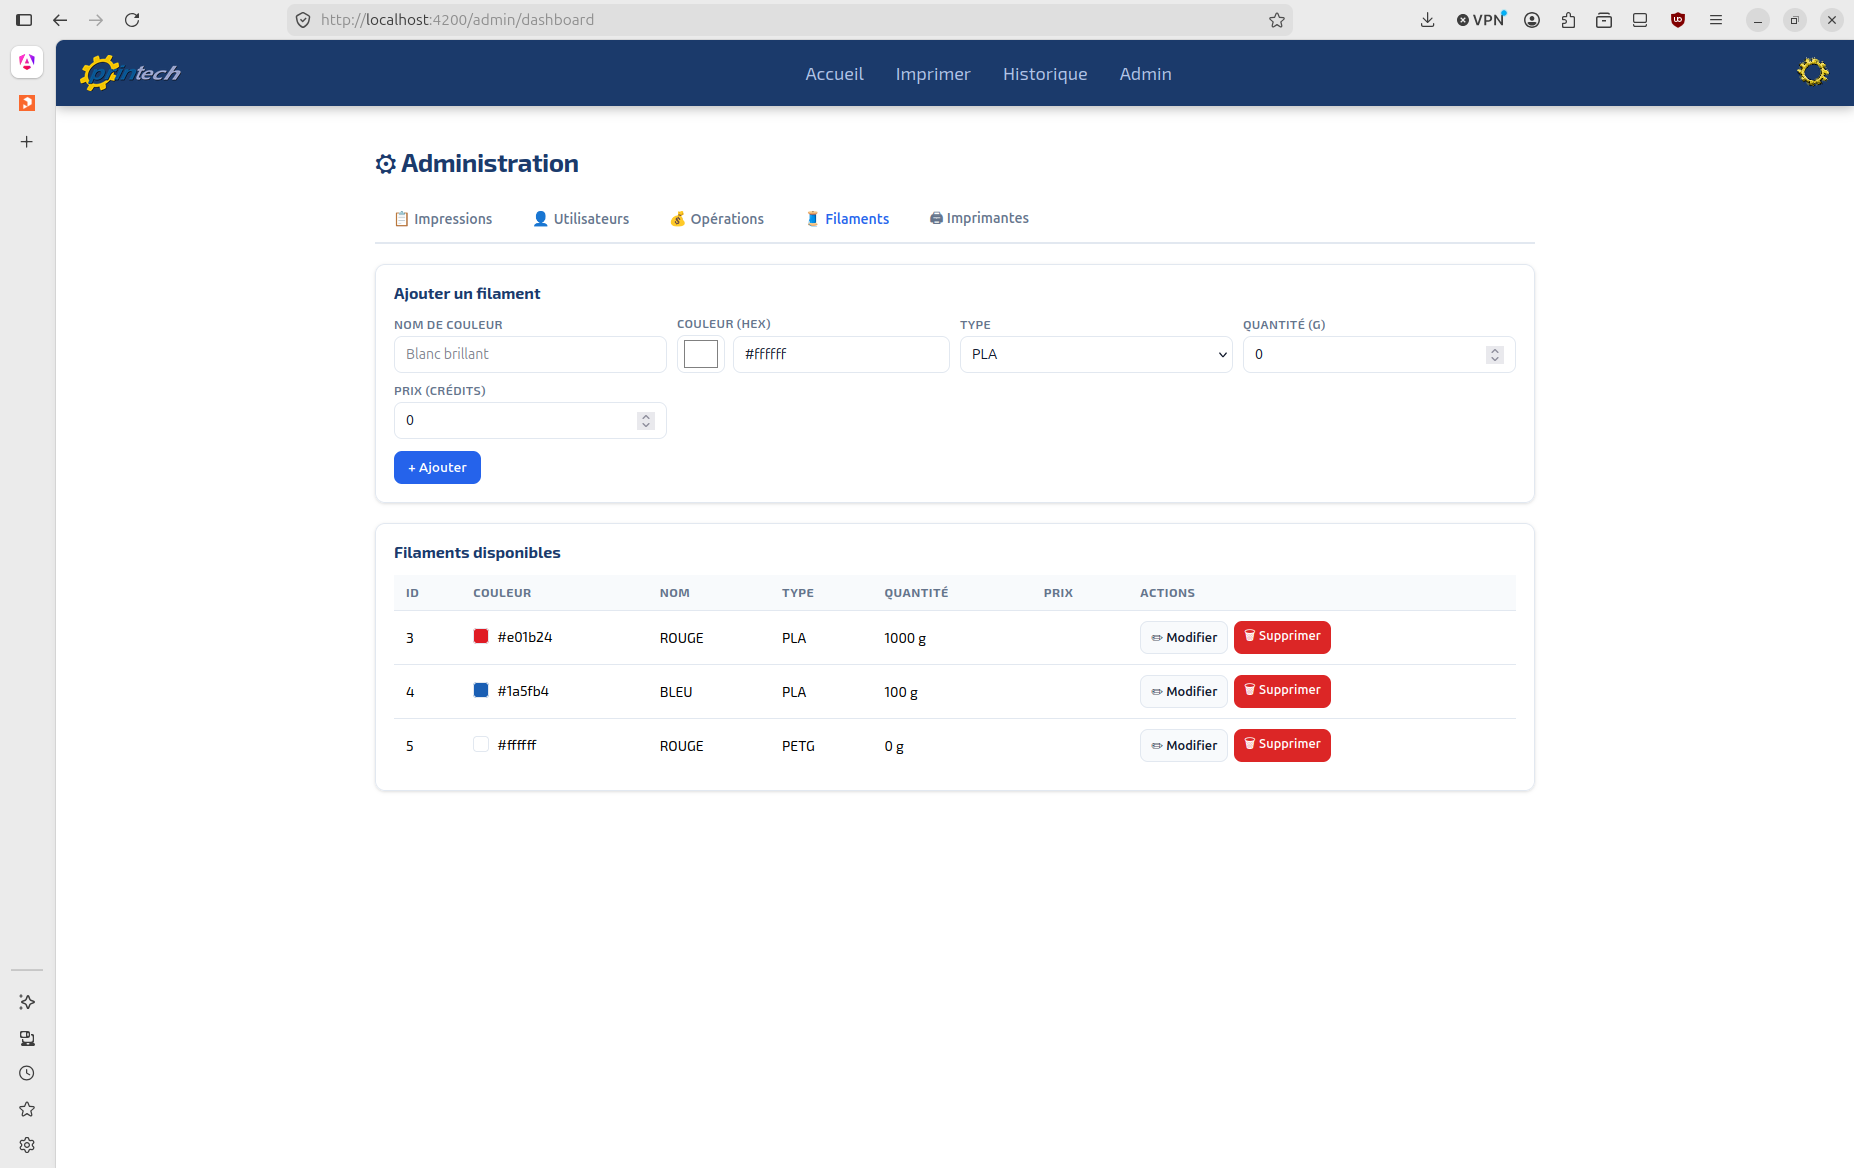
\includegraphics{screenshots/admin-filaments.png}\\
  Vue dédiée au contrôle des stocks de plastique (Fonctionnalité
  \textbf{F07 : Gestion des filaments}). Elle permet d'enregistrer les
  nouvelles bobines, de surveiller la quantité de matière restante en
  grammes (\textbf{F07-2}).
\item
  \textbf{Suivi financier et des transactions}
  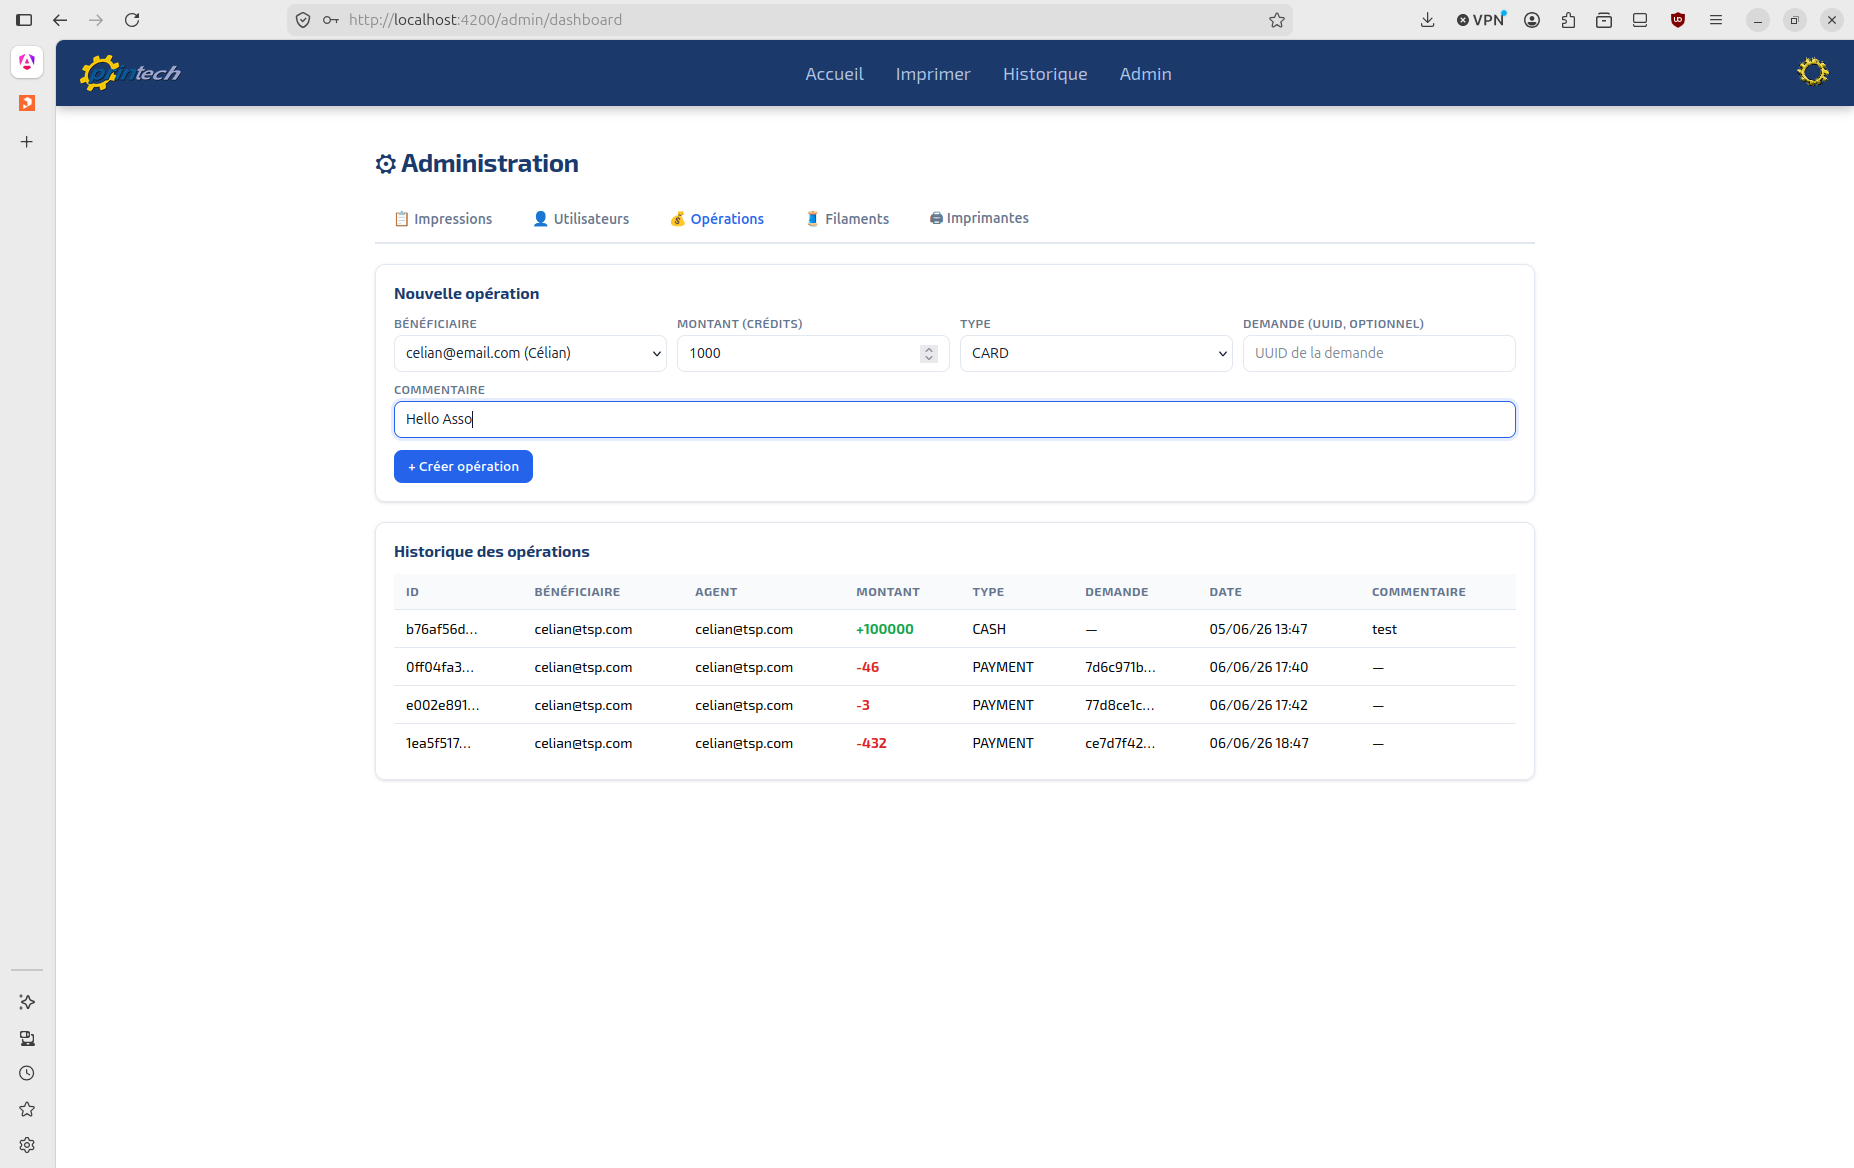
\includegraphics{screenshots/admin-operations.png}\\
  Historique financier de la plateforme (Fonctionnalité \textbf{F04-4 :
  Gestion crédit}). Cet écran liste de manière chronologique tous les
  débits, les rechargements HelloAsso fructueux ainsi que les
  remboursements automatiques émis suite à une erreur d'impression.
\item
  \textbf{Administration des comptes utilisateurs}
  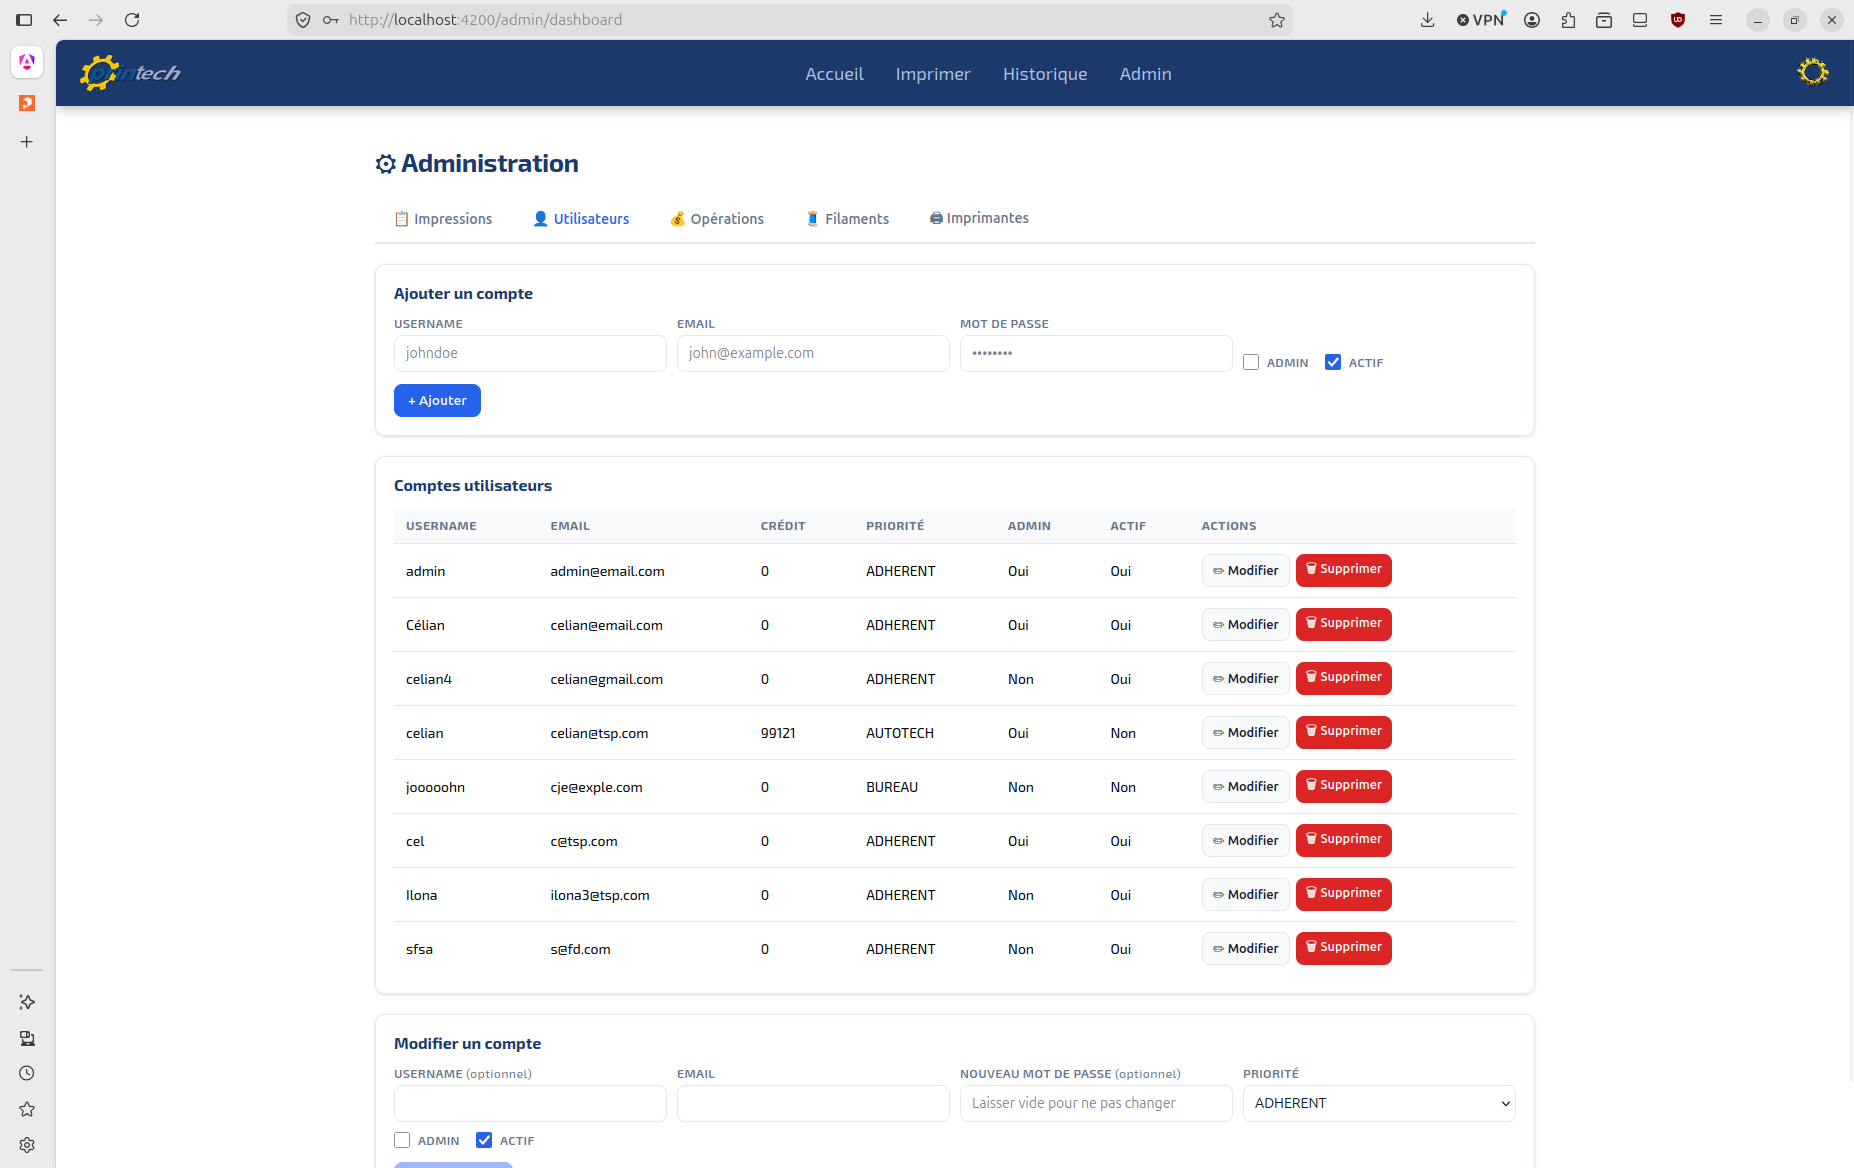
\includegraphics{screenshots/admin-users.png}\\
  Interface de modération des profils (Fonctionnalité \textbf{F04-1}).
  Elle permet également de modifier les rôles (adhérents, bureau, membre
  projet) (\textbf{F03-5}). ---
\end{itemize}

\newpage

\hypertarget{validation-et-tests}{%
\section{5. Validation et tests}\label{validation-et-tests}}

Pour garantir la robustesse de l'application PrINTech, nous avons mis en
place une stratégie de tests automatisés. L'effort principal a été
concentré sur la validation fonctionnelle du backend (Django), complété
par des mécanismes de tests d'intégration et d'interface (Playwright).

\hypertarget{tests-backend-django}{%
\subsection{5.1. Tests Backend (Django)}\label{tests-backend-django}}

Le backend constituant le cœur logique et financier de notre application
(notamment avec la gestion du crédit des utilisateurs), nous avons conçu
une suite de nombreux tests unitaires et d'intégration rigoureuse à
l'aide du framework de test de \emph{Django REST Framework}
(\texttt{APITestCase}). Les tests se trouvent dans le fichier
\texttt{PrINTech-Back/back/apps/api/tests.py}

\hypertarget{exemples}{%
\subsubsection{5.1.1. Exemples:}\label{exemples}}

Une attention particulière a été portée à la sécurité et à l'étanchéité
des droits entre les utilisateurs réguliers et les administrateurs du
bureau INTech. \textbf{Accès aux ressources critiques} : Nous testons
systématiquement qu'un utilisateur standard reçoit une erreur
\texttt{HTTP\_403\_FORBIDDEN} lorsqu'il tente de modifier l'état d'une
imprimante (endpoint \texttt{admin-detail}), alors qu'un jeton
d'administrateur valide la requête avec un statut
\texttt{HTTP\_200\_OK}.

\textbf{Calcul automatique de la consommation} : Les tests valident que
l'API calcule correctement le poids total de plastique consommé en
multipliant le nombre d'impressions demandées par le poids unitaire de
la pièce.

\textbf{Débit du solde utilisateur} : Nous nous assurons qu'à la
soumission d'un fichier STL valide, le crédit de l'étudiant est
immédiatement débité au prorata de la quantité et du type de filament
choisi (ex: passage d'une balance initiale de 100 unités à une valeur
calculée résiduelle).

\textbf{Isolation des requêtes} : Nos cas de tests
(\texttt{test\_user\_can\_only\_see\_their\_own\_requests}) certifient
qu'un utilisateur connecté ne peut en aucun cas interroger ou lister les
fichiers et demandes d'un autre étudiant, prévenant ainsi toute fuite de
données.

\begin{center}\rule{0.5\linewidth}{0.5pt}\end{center}

\hypertarget{tests-dinterface-playwright-et-validation-frontend}{%
\subsection{5.2. Tests d'Interface (Playwright) et Validation
Frontend}\label{tests-dinterface-playwright-et-validation-frontend}}

Pour la partie émergée de l'iceberg (le Frontend), l'objectif initial
intégrait le déploiement de tests de bout en bout (E2E) via l'outil
\textbf{Playwright}.

Cependant, comme évoqué dans notre bilan de projet (Section 6.1.3), le
retard accumulé sur l'apprentissage d'Angular et la complexité de
l'interfaçage asynchrone ont limité la couverture finale de ces tests
E2E.

\newpage

\hypertarget{bilan-du-projet}{%
\section{6. Bilan du projet}\label{bilan-du-projet}}

\hypertarget{plannings}{%
\subsection{6.1. Plannings}\label{plannings}}

On a eu de nombreux retards sur le projet, notamment à cause de la
participation de certains membres de notre équipe à la coupe de France
de Robotique dans le cadre du GATE. On a également sous-estimé la
difficulté d'apprentissage des technologies utilisés (Angular et
Django). On était pas tous capable de faire à la fois du frontend et du
backend ce qui a crée des complications. De plus Arnaud qui était censé
implémenté la communication avec les imprimantes n'a pas réussi ce qui a
fortement limité le projet.

\hypertarget{planning-pruxe9visionnel}{%
\subsubsection{6.1.1. Planning
prévisionnel}\label{planning-pruxe9visionnel}}

\begin{figure}
\centering
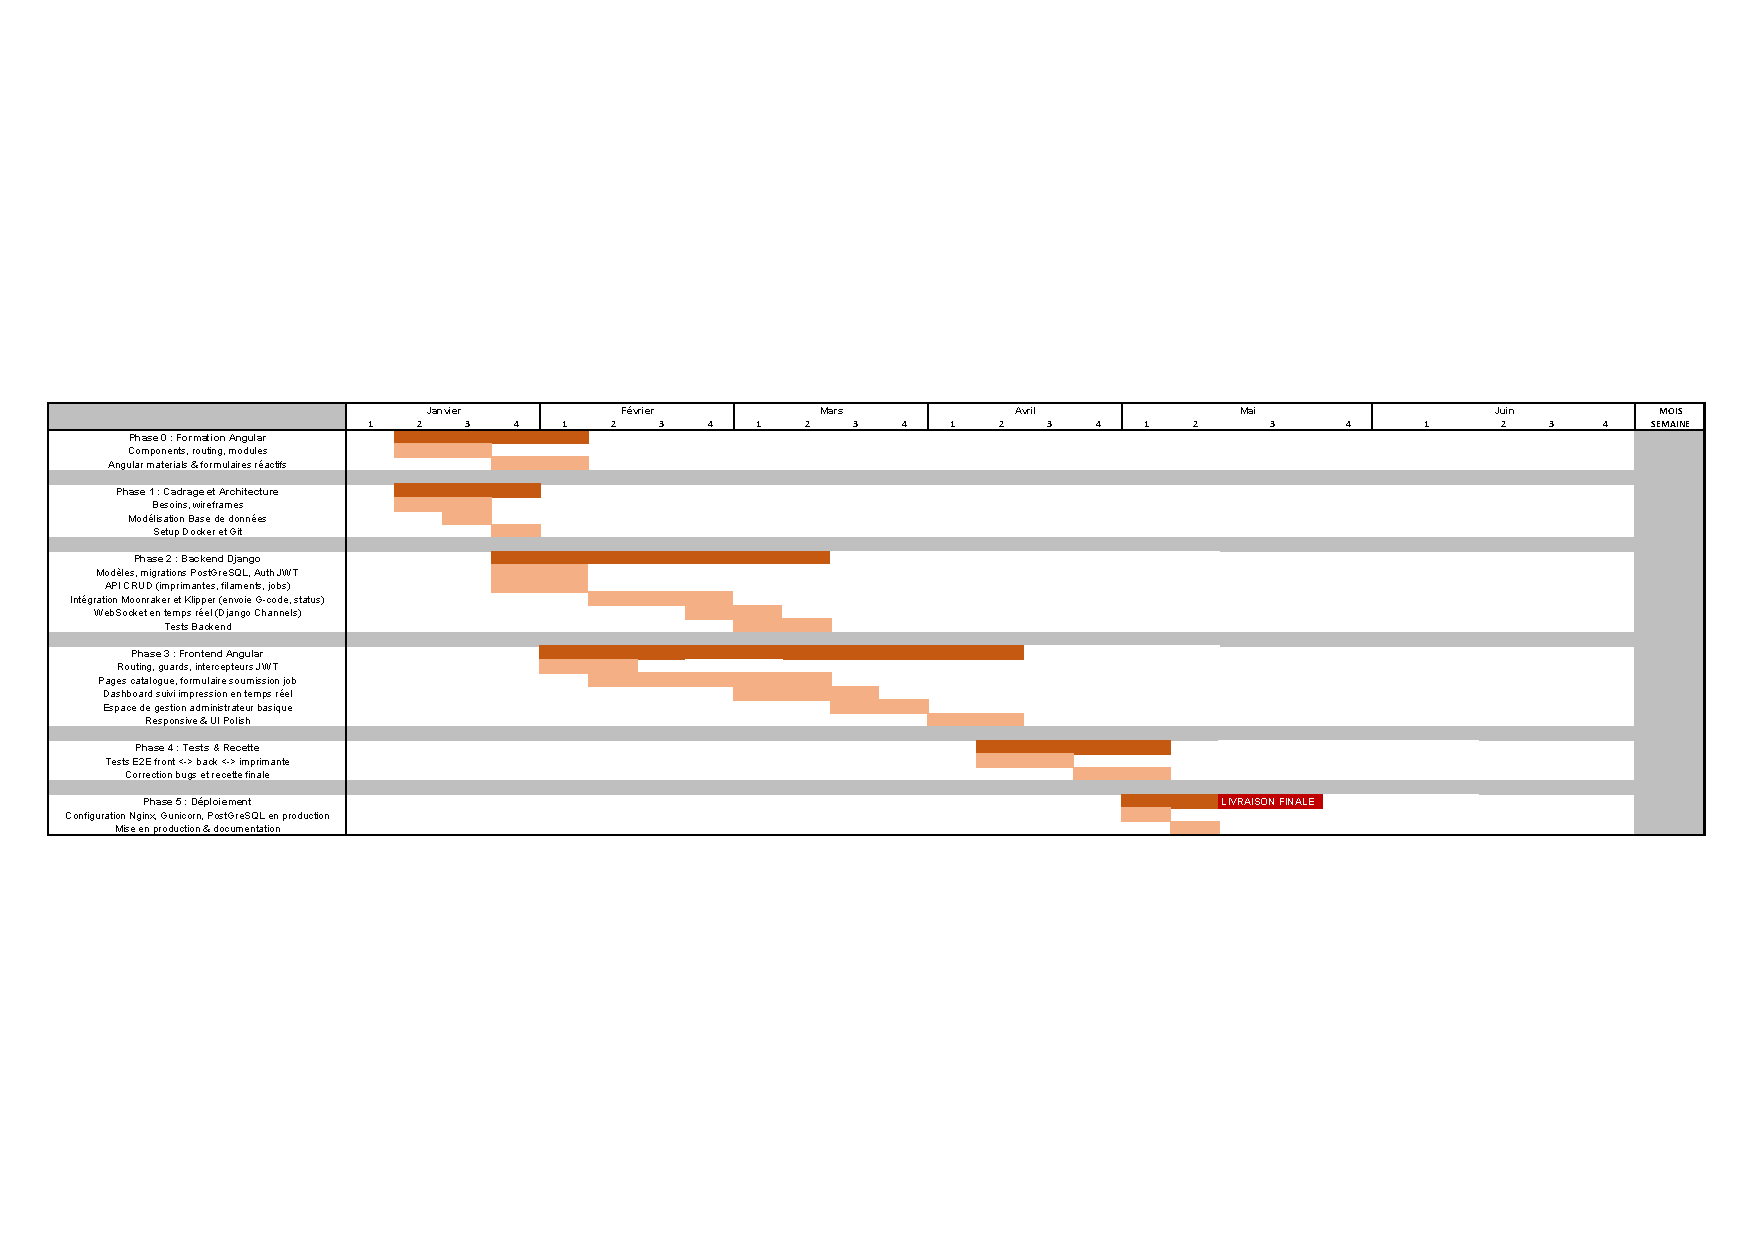
\includegraphics{planning-previsionnel.pdf}
\caption{Planning prévisionnel du projet PrIntech}
\end{figure}

\begin{center}\rule{0.5\linewidth}{0.5pt}\end{center}

\newpage

\hypertarget{planning-final}{%
\subsubsection{6.1.2. Planning final}\label{planning-final}}

\begin{figure}
\centering
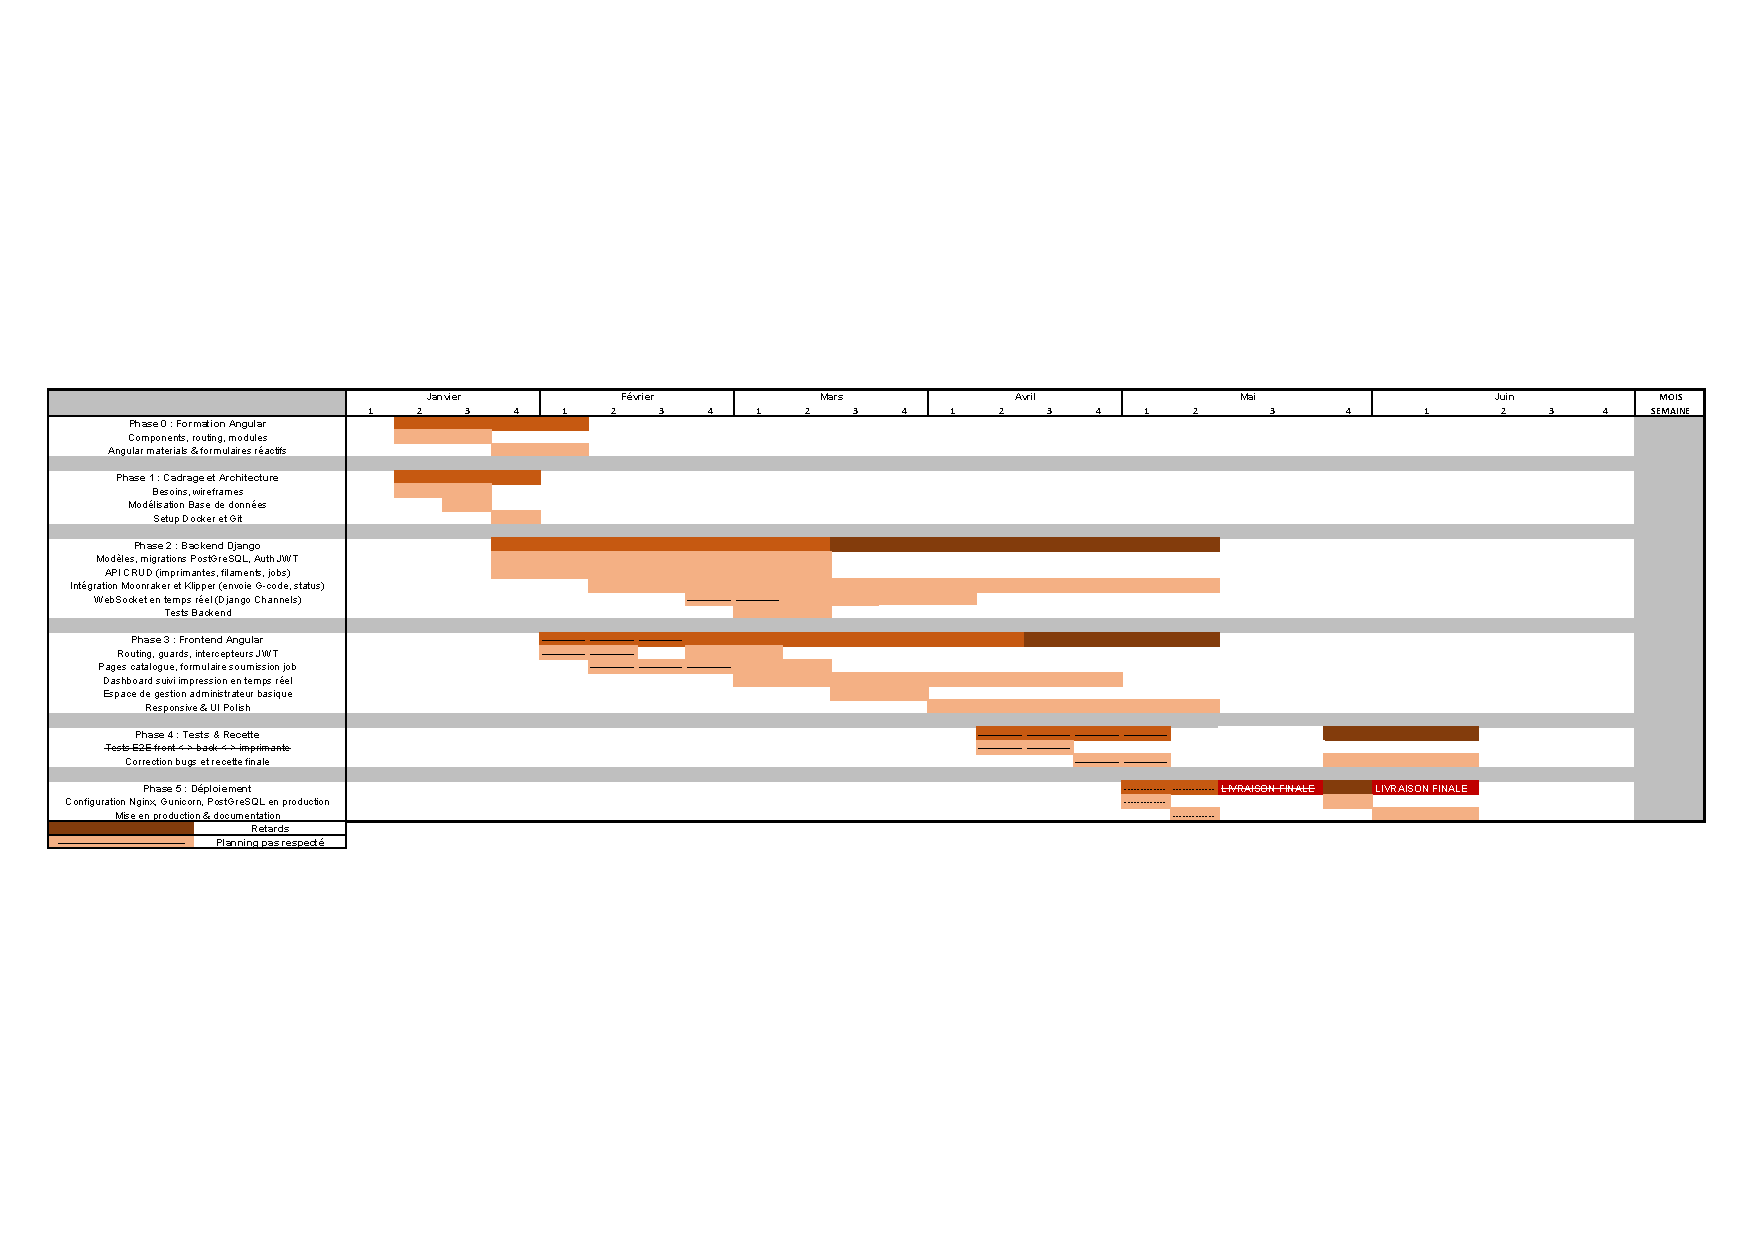
\includegraphics{planning-final.pdf}
\caption{Planning final du projet PrIntech}
\end{figure}

\begin{center}\rule{0.5\linewidth}{0.5pt}\end{center}

\newpage

\hypertarget{commentaires}{%
\subsubsection{6.1.3. Commentaires}\label{commentaires}}

\begin{itemize}
\item
  \textbf{Choix du planning prévisionnel} :

  \begin{itemize}
  \tightlist
  \item
    Angular est appris en parallele du projet. Le dev front ne commence
    qu'en fevrier.
  \item
    Django est maitrise -\textgreater{} execution rapide. La partie
    Moonraker/Klipper est la plus incertaine.
  \item
    la phase 3 est la plus longue a cause de l'apprentissage en cours.
  \end{itemize}
\item
  \textbf{Comparaison au planning réel} :

  \begin{itemize}
  \tightlist
  \item
    le projet a accumulé du retard notamment en raison d'autres dates
    importantes comme les projets Gate ou bien les partiels mais aussi
    car on a sous-estimé la complexité de certaines taches que nous
    verrons plus bas.
  \item
    en réponse, on a ré-évalué le périmètre de notre projet afin d'en
    inclure à la date du rendu que les fonctionnalités nécessaires au vu
    du cahier des charges (Pas de tests e2e pour l'instant)
  \item
    Ce retard n'est pas une fatalité puisque compte tenu de l'utilité du
    projet, celui-ci sera poursuivi à bien au-delà de la date de rendu.
  \end{itemize}
\end{itemize}

\begin{center}\rule{0.5\linewidth}{0.5pt}\end{center}

\newpage

\hypertarget{plan-de-charges}{%
\subsection{6.2. Plan de charges}\label{plan-de-charges}}

L'écart le plus marquant entre notre planification et la réalité réside
dans la courbe d'apprentissage des technologies choisies (Angular et
Django), qui s'est révélée bien plus longue et abrupte que prévu.
N'ayant pas de compétences approfondies préalables sur ces frameworks,
l'assimilation de concepts a pris plus de temps que prévu.

\hypertarget{plan-de-charges-pruxe9visionnel-et-final}{%
\subsubsection{6.2.1. Plan de charges prévisionnel et
final}\label{plan-de-charges-pruxe9visionnel-et-final}}

\begin{figure}
\centering
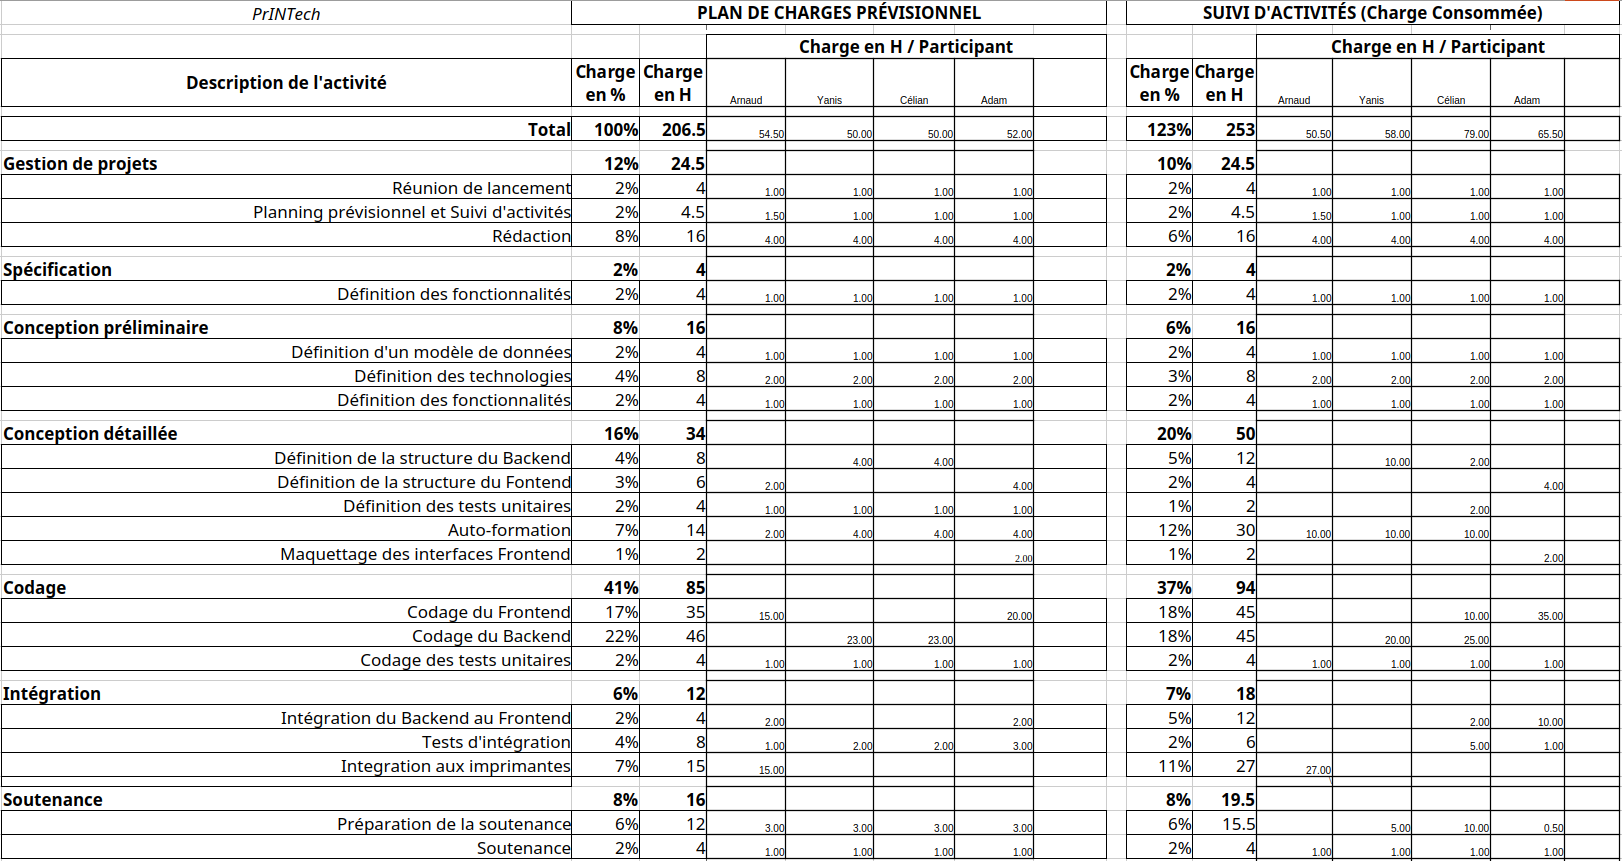
\includegraphics{planChargeSuiviActivites.png}
\caption{Plan de Charge}
\end{figure}

\begin{center}\rule{0.5\linewidth}{0.5pt}\end{center}

\newpage

\hypertarget{commentaires-1}{%
\subsubsection{6.2.3. Commentaires}\label{commentaires-1}}

Nous avons bien utilisé le temps imparti. Celui-ci nous a permis de nous
former non seulement sur les technologies auxquelles nous étions
assignées mais aussi à comprendre l'ensemble du code que ce soit le
front ou le back.

Nous sommes ainsi parvenu à rendre notre profil beaucoup plus attractif
avec une compréhension plus fine des abstractions des différentes
technologies mais aussi une vision beaucoup moins étroite de notre champ
d'action.

Pour indication, Célian ne connaissait pas Django au démarrage du
projet, Adam démarrait sur Angular et Yanis était surtout focalisé sur
Django; maintenant, nous sommes tous en mesure de comprendre le code de
l'autre et de le corriger à travers un système de PR (Pull Request) sur
Git.

\begin{center}\rule{0.5\linewidth}{0.5pt}\end{center}

\newpage

\hypertarget{difficultuxe9s-rencontruxe9es}{%
\subsection{6.3. Difficultés
rencontrées}\label{difficultuxe9s-rencontruxe9es}}

Notre projet, malgré un produit final assez satisfaisant, a été le
théâtres de certaines difficultés qui nous ont poussé à modifier notre
champ d'action :

\begin{itemize}
\item
  La mise en commun du travail a été plus nébuleuse que prévu (notamment
  après l'instauration de PR qui ont empêchés le bon fonctionnement de
  certaines commandes de git flow)
\item
  les retards accumulés qui on sappé l'efficacité du projet malgré un
  démarrage rapide
\item
  l'utilisation des APIs des imprimantes 3D : Notre objectif initial
  était de relier directement les imprimantes 3D à l'application grâce
  au logiciel FDM Monster. Cependant, cette configuration s'est révélée
  difficile en raison des systèmes propriétaires des machines. De plus,
  comme les imprimantes sont très sollicitées, nous avons temporairement
  configuré le site pour qu'un administrateur lance chaque impression
  manuellement. Nous continuons néanmoins à travailler sur
  l'automatisation de ce processus.
\end{itemize}

\hypertarget{fonctionalituxe9s-ruxe9alisuxe9-ou-pas}{%
\subsubsection{6.3.1 Fonctionalités réalisé ou
pas}\label{fonctionalituxe9s-ruxe9alisuxe9-ou-pas}}

\begin{longtable}[]{@{}
  >{\raggedright\arraybackslash}p{(\columnwidth - 8\tabcolsep) * \real{0.1818}}
  >{\raggedright\arraybackslash}p{(\columnwidth - 8\tabcolsep) * \real{0.1818}}
  >{\raggedright\arraybackslash}p{(\columnwidth - 8\tabcolsep) * \real{0.1818}}
  >{\centering\arraybackslash}p{(\columnwidth - 8\tabcolsep) * \real{0.2273}}
  >{\centering\arraybackslash}p{(\columnwidth - 8\tabcolsep) * \real{0.2273}}@{}}
\toprule\noalign{}
\begin{minipage}[b]{\linewidth}\raggedright
ID
\end{minipage} & \begin{minipage}[b]{\linewidth}\raggedright
Fonctionnalité de l'application
\end{minipage} & \begin{minipage}[b]{\linewidth}\raggedright
Description technique
\end{minipage} & \begin{minipage}[b]{\linewidth}\centering
Priorité
\end{minipage} & \begin{minipage}[b]{\linewidth}\centering
Statut
\end{minipage} \\
\midrule\noalign{}
\endhead
\bottomrule\noalign{}
\endlastfoot
\textbf{F01} & \textbf{Authentification} & Connexion et déconnexion. &
Haute & \textbf{Réalisé} \\
\textbf{F02} & \textbf{Gestion des profils} & Affichage et modification
des informations utilisateurs. & Basse & \textbf{Réalisé} \\
\textbf{F03} & \textbf{Gestion des impressions} & Flux complet
d'impression 3D, du dépôt STL à la mise en file. & Haute &
\textbf{Réalisé} \\
\textbf{F03-1} & \textbf{Déposer un STL} & Upload d'un fichier STL. &
Haute & \textbf{Réalisé} \\
\textbf{F03-2} & \textbf{Slicer automatique} & Convertir le modèle en
G-code via un slicer. & Moyenne & \textbf{Non réalisé} \\
\textbf{F03-3} & \textbf{Estimation du coût} & Calculer le prix
d'impression à partir des paramètres. & Basse & \textbf{Non réalisé} \\
\textbf{F03-4} & \textbf{Position dans la file} & Afficher la place du
travail dans la file. & Basse & \textbf{Non réalisé} \\
\textbf{F03-5} & \textbf{Priorité projets INTech} & Rôle dédié pour
prioriser les impressions. & Basse & \textbf{Réalisé} \\
\textbf{F03-6} & \textbf{Crédit restant} & Afficher le crédit restant
d'un utilisateur. & Basse & \textbf{Réalisé} \\
\textbf{F03-7} & \textbf{Quantité d'impressions} & Indiquer le nombre
d'exemplaires à imprimer. & Basse & \textbf{Réalisé} \\
\textbf{F04} & \textbf{Espace administrateur} & Interface
d'administration pour une gestion complète. & Moyenne &
\textbf{Réalisé} \\
\textbf{F04-1} & \textbf{Gestion des utilisateurs} & Créer, modifier et
supprimer les utilisateurs. & Haute & \textbf{Réalisé} \\
\textbf{F04-2} & \textbf{Gestion des travaux} & Créer, modifier et
supprimer la file de travaux. & Moyenne & \textbf{Réalisé} \\
\textbf{F04-3} & \textbf{Reprise des erreurs} & Déclarer un travail en
erreur et le remettre en file. & Moyenne & \textbf{Non réalisé} \\
\textbf{F04-4} & \textbf{Gestion crédit} & Gestion des crédits des
utilisateurs (recharge). & Haute & \textbf{Réalisé} \\
\textbf{F05} & \textbf{Intégrations} & SSO et notifications externes. &
Optionnelle & \textbf{Non réalisé} \\
\textbf{F05-1} & \textbf{Intégration CAS} & Inscription et connexion via
le CAS de l'école. & Optionnelle & \textbf{Non réalisé} \\
\textbf{F05-2} & \textbf{Intégration Discord} & Utiliser des webhooks
pour les notifications. & Optionnelle & \textbf{Non réalisé} \\
\textbf{F05-3} & \textbf{Intégration HelloAsso} & Créditer les comptes
via HelloAsso. & Optionnelle & \textbf{Non réalisé} \\
\textbf{F06} & \textbf{Impression technique} & Options avancées
d'impression. & Optionnelle & \textbf{Non réalisé} \\
\textbf{F06-1} & \textbf{Utilisation de supports} & Détecter la
nécessité de supports. & Optionnelle & \textbf{Non réalisé} \\
\textbf{F06-2} & \textbf{Paramétrage du slicer} & Permettre l'upload
d'un JSON de paramètres. & Optionnelle & \textbf{Non réalisé} \\
\textbf{F06-3} & \textbf{Choix des matériaux} & Choisir un plastique
autre que le PLA. & Optionnelle & \textbf{Réalisé} \\
\textbf{F07} & \textbf{Gestion des filaments} & Administration des
filaments et du stock. & Optionnelle & \textbf{Réalisé} \\
\textbf{F07-1} & \textbf{Activation des filaments} & Activer et
désactiver des filaments. & Optionnelle & \textbf{Non réalisé} \\
\textbf{F07-2} & \textbf{Gestion du filament} & Gérer la quantité de
filament restant. & Optionnelle & \textbf{Réalisé} \\
\textbf{F07-3} & \textbf{Gestion de consommation} & Rapport sur
quantités, crédits et montant. & Optionnelle & \textbf{réalisé} \\
\end{longtable}

\begin{center}\rule{0.5\linewidth}{0.5pt}\end{center}

\newpage

\hypertarget{conclusion-et-perspective}{%
\section{7. Conclusion et perspective}\label{conclusion-et-perspective}}

Malgré des difficultés, notre projet a produit une Application Web
fonctionnelle selon les critères que nous nous étions imposés en
préambule avec le cahier des charges.

Tout du moins, nous souhaiterions peaufiner ce projet au-delà du rendu
final, que ce soit par la continuation de celui-ci par un autre groupe
de projet informatique, ou bien par la maintenance de celui-ci par
l'Association Intech elle-même. Il faudra donc le déployer ce qu'on a
pas encore pu faire. On pense utilisé une machine virtuelle fournie par
l'association Minet. À terme il pourra être réellement utilisé par
l'association.

Ce projet est un projet enrichissant pour un étudiant ingénieur dans le
développement informatique à travers l'utilisation d'outils et de
technologies professionnels qui s'intègre pleinement dans le cadre de
nos études et du campus avec Intech.

Ce projet, au-delà de la réalisation purement technique, est aussi une
expérience d'équipe avec tout ses avantages et ses défauts qu'on a
expérimenté (comme les retards et la mise en commun du code). Cela en
fait donc une force pour tous nos futurs projets en groupe.

\begin{center}\rule{0.5\linewidth}{0.5pt}\end{center}
